\documentclass[twoside]{book}

% Packages required by doxygen
\usepackage{fixltx2e}
\usepackage{calc}
\usepackage{doxygen}
\usepackage[export]{adjustbox} % also loads graphicx
\usepackage{graphicx}
\usepackage[utf8]{inputenc}
\usepackage{makeidx}
\usepackage{multicol}
\usepackage{multirow}
\PassOptionsToPackage{warn}{textcomp}
\usepackage{textcomp}
\usepackage[nointegrals]{wasysym}
\usepackage[table]{xcolor}

% Font selection
\usepackage[T1]{fontenc}
\usepackage[scaled=.90]{helvet}
\usepackage{courier}
\usepackage{amssymb}
\usepackage{sectsty}
\renewcommand{\familydefault}{\sfdefault}
\allsectionsfont{%
  \fontseries{bc}\selectfont%
  \color{darkgray}%
}
\renewcommand{\DoxyLabelFont}{%
  \fontseries{bc}\selectfont%
  \color{darkgray}%
}
\newcommand{\+}{\discretionary{\mbox{\scriptsize$\hookleftarrow$}}{}{}}

% Page & text layout
\usepackage{geometry}
\geometry{%
  a4paper,%
  top=2.5cm,%
  bottom=2.5cm,%
  left=2.5cm,%
  right=2.5cm%
}
\tolerance=750
\hfuzz=15pt
\hbadness=750
\setlength{\emergencystretch}{15pt}
\setlength{\parindent}{0cm}
\setlength{\parskip}{3ex plus 2ex minus 2ex}
\makeatletter
\renewcommand{\paragraph}{%
  \@startsection{paragraph}{4}{0ex}{-1.0ex}{1.0ex}{%
    \normalfont\normalsize\bfseries\SS@parafont%
  }%
}
\renewcommand{\subparagraph}{%
  \@startsection{subparagraph}{5}{0ex}{-1.0ex}{1.0ex}{%
    \normalfont\normalsize\bfseries\SS@subparafont%
  }%
}
\makeatother

% Headers & footers
\usepackage{fancyhdr}
\pagestyle{fancyplain}
\fancyhead[LE]{\fancyplain{}{\bfseries\thepage}}
\fancyhead[CE]{\fancyplain{}{}}
\fancyhead[RE]{\fancyplain{}{\bfseries\leftmark}}
\fancyhead[LO]{\fancyplain{}{\bfseries\rightmark}}
\fancyhead[CO]{\fancyplain{}{}}
\fancyhead[RO]{\fancyplain{}{\bfseries\thepage}}
\fancyfoot[LE]{\fancyplain{}{}}
\fancyfoot[CE]{\fancyplain{}{}}
\fancyfoot[RE]{\fancyplain{}{\bfseries\scriptsize Generated by Doxygen }}
\fancyfoot[LO]{\fancyplain{}{\bfseries\scriptsize Generated by Doxygen }}
\fancyfoot[CO]{\fancyplain{}{}}
\fancyfoot[RO]{\fancyplain{}{}}
\renewcommand{\footrulewidth}{0.4pt}
\renewcommand{\chaptermark}[1]{%
  \markboth{#1}{}%
}
\renewcommand{\sectionmark}[1]{%
  \markright{\thesection\ #1}%
}

% Indices & bibliography
\usepackage{natbib}
\usepackage[titles]{tocloft}
\setcounter{tocdepth}{3}
\setcounter{secnumdepth}{5}
\makeindex

% Hyperlinks (required, but should be loaded last)
\usepackage{ifpdf}
\ifpdf
  \usepackage[pdftex,pagebackref=true]{hyperref}
\else
  \usepackage[ps2pdf,pagebackref=true]{hyperref}
\fi
\hypersetup{%
  colorlinks=true,%
  linkcolor=blue,%
  citecolor=blue,%
  unicode%
}

% Custom commands
\newcommand{\clearemptydoublepage}{%
  \newpage{\pagestyle{empty}\cleardoublepage}%
}

\usepackage{caption}
\captionsetup{labelsep=space,justification=centering,font={bf},singlelinecheck=off,skip=4pt,position=top}

%===== C O N T E N T S =====

\begin{document}

% Titlepage & ToC
\hypersetup{pageanchor=false,
             bookmarksnumbered=true,
             pdfencoding=unicode
            }
\pagenumbering{alph}
\begin{titlepage}
\vspace*{7cm}
\begin{center}%
{\Large Zombie\+Survival }\\
\vspace*{1cm}
{\large Generated by Doxygen 1.8.14}\\
\end{center}
\end{titlepage}
\clearemptydoublepage
\pagenumbering{roman}
\tableofcontents
\clearemptydoublepage
\pagenumbering{arabic}
\hypersetup{pageanchor=true}

%--- Begin generated contents ---
\chapter{Namespace Index}
\section{Packages}
Here are the packages with brief descriptions (if available)\+:\begin{DoxyCompactList}
\item\contentsline{section}{\mbox{\hyperlink{namespace_game2}{Game2}} }{\pageref{namespace_game2}}{}
\item\contentsline{section}{\mbox{\hyperlink{namespace_solar_battle}{Solar\+Battle}} }{\pageref{namespace_solar_battle}}{}
\item\contentsline{section}{\mbox{\hyperlink{namespace_solar_battle_1_1_camera}{Solar\+Battle.\+Camera}} }{\pageref{namespace_solar_battle_1_1_camera}}{}
\end{DoxyCompactList}

\chapter{Hierarchical Index}
\section{Class Hierarchy}
This inheritance list is sorted roughly, but not completely, alphabetically\+:\begin{DoxyCompactList}
\item Animated\+Game\+Object\begin{DoxyCompactList}
\item \contentsline{section}{Game2.\+Blood}{\pageref{class_game2_1_1_blood}}{}
\item \contentsline{section}{Game2.\+Blood\+Effect}{\pageref{class_game2_1_1_blood_effect}}{}
\item \contentsline{section}{Game2.\+Player}{\pageref{class_game2_1_1_player}}{}
\item \contentsline{section}{Game2.\+Player\+Blood}{\pageref{class_game2_1_1_player_blood}}{}
\end{DoxyCompactList}
\item Game\begin{DoxyCompactList}
\item \contentsline{section}{Game2.\+Game\+World}{\pageref{class_game2_1_1_game_world}}{}
\end{DoxyCompactList}
\item \contentsline{section}{Game2.\+Game\+Object}{\pageref{class_game2_1_1_game_object}}{}
\begin{DoxyCompactList}
\item \contentsline{section}{Game2.\+Boss}{\pageref{class_game2_1_1_boss}}{}
\item \contentsline{section}{Game2.\+Bullet}{\pageref{class_game2_1_1_bullet}}{}
\item \contentsline{section}{Game2.\+Enemy}{\pageref{class_game2_1_1_enemy}}{}
\end{DoxyCompactList}
\item \contentsline{section}{Game2.\+Game\+Over\+Menu\+Screen}{\pageref{class_game2_1_1_game_over_menu_screen}}{}
\item \contentsline{section}{Game2.\+Game\+Timer}{\pageref{class_game2_1_1_game_timer}}{}
\item \contentsline{section}{Solar\+Battle.\+Camera.\+Player\+Camera}{\pageref{class_solar_battle_1_1_camera_1_1_player_camera}}{}
\item \contentsline{section}{Game2.\+test}{\pageref{class_game2_1_1test}}{}
\end{DoxyCompactList}

\chapter{Class Index}
\section{Class List}
Here are the classes, structs, unions and interfaces with brief descriptions\+:\begin{DoxyCompactList}
\item\contentsline{section}{\mbox{\hyperlink{class_game2_1_1_blood}{Game2.\+Blood}} }{\pageref{class_game2_1_1_blood}}{}
\item\contentsline{section}{\mbox{\hyperlink{class_game2_1_1_blood_effect}{Game2.\+Blood\+Effect}} }{\pageref{class_game2_1_1_blood_effect}}{}
\item\contentsline{section}{\mbox{\hyperlink{class_game2_1_1_boss}{Game2.\+Boss}} \\*Class that represents a boss }{\pageref{class_game2_1_1_boss}}{}
\item\contentsline{section}{\mbox{\hyperlink{class_game2_1_1_bullet}{Game2.\+Bullet}} \\*Class that represents a \mbox{\hyperlink{class_game2_1_1_bullet}{Bullet}} fired from the player }{\pageref{class_game2_1_1_bullet}}{}
\item\contentsline{section}{\mbox{\hyperlink{class_game2_1_1_enemy}{Game2.\+Enemy}} \\*Class that represents a zombie }{\pageref{class_game2_1_1_enemy}}{}
\item\contentsline{section}{\mbox{\hyperlink{class_game2_1_1_game_object}{Game2.\+Game\+Object}} }{\pageref{class_game2_1_1_game_object}}{}
\item\contentsline{section}{\mbox{\hyperlink{class_game2_1_1_game_over_menu_screen}{Game2.\+Game\+Over\+Menu\+Screen}} }{\pageref{class_game2_1_1_game_over_menu_screen}}{}
\item\contentsline{section}{\mbox{\hyperlink{class_game2_1_1_game_timer}{Game2.\+Game\+Timer}} \\*Class that represents a game time to set waves }{\pageref{class_game2_1_1_game_timer}}{}
\item\contentsline{section}{\mbox{\hyperlink{class_game2_1_1_game_world}{Game2.\+Game\+World}} \\*This is the main type for your game. }{\pageref{class_game2_1_1_game_world}}{}
\item\contentsline{section}{\mbox{\hyperlink{class_game2_1_1_player}{Game2.\+Player}} \\*Class that represents the player }{\pageref{class_game2_1_1_player}}{}
\item\contentsline{section}{\mbox{\hyperlink{class_game2_1_1_player_blood}{Game2.\+Player\+Blood}} }{\pageref{class_game2_1_1_player_blood}}{}
\item\contentsline{section}{\mbox{\hyperlink{class_solar_battle_1_1_camera_1_1_player_camera}{Solar\+Battle.\+Camera.\+Player\+Camera}} }{\pageref{class_solar_battle_1_1_camera_1_1_player_camera}}{}
\item\contentsline{section}{\mbox{\hyperlink{class_game2_1_1test}{Game2.\+test}} }{\pageref{class_game2_1_1test}}{}
\end{DoxyCompactList}

\chapter{File Index}
\section{File List}
Here is a list of all files with brief descriptions\+:\begin{DoxyCompactList}
\item\contentsline{section}{\mbox{\hyperlink{_animated_game_object_8cs}{Animated\+Game\+Object.\+cs}} }{\pageref{_animated_game_object_8cs}}{}
\item\contentsline{section}{\mbox{\hyperlink{_blood_8cs}{Blood.\+cs}} }{\pageref{_blood_8cs}}{}
\item\contentsline{section}{\mbox{\hyperlink{_blood_effect_8cs}{Blood\+Effect.\+cs}} }{\pageref{_blood_effect_8cs}}{}
\item\contentsline{section}{\mbox{\hyperlink{_boss_8cs}{Boss.\+cs}} }{\pageref{_boss_8cs}}{}
\item\contentsline{section}{\mbox{\hyperlink{_bullet_8cs}{Bullet.\+cs}} }{\pageref{_bullet_8cs}}{}
\item\contentsline{section}{\mbox{\hyperlink{_enemy_8cs}{Enemy.\+cs}} }{\pageref{_enemy_8cs}}{}
\item\contentsline{section}{\mbox{\hyperlink{_game_object_8cs}{Game\+Object.\+cs}} }{\pageref{_game_object_8cs}}{}
\item\contentsline{section}{\mbox{\hyperlink{_game_over_menu_screen_8cs}{Game\+Over\+Menu\+Screen.\+cs}} }{\pageref{_game_over_menu_screen_8cs}}{}
\item\contentsline{section}{\mbox{\hyperlink{_game_timer_8cs}{Game\+Timer.\+cs}} }{\pageref{_game_timer_8cs}}{}
\item\contentsline{section}{\mbox{\hyperlink{_game_world_8cs}{Game\+World.\+cs}} }{\pageref{_game_world_8cs}}{}
\item\contentsline{section}{\mbox{\hyperlink{_player_8cs}{Player.\+cs}} }{\pageref{_player_8cs}}{}
\item\contentsline{section}{\mbox{\hyperlink{_player_blood_8cs}{Player\+Blood.\+cs}} }{\pageref{_player_blood_8cs}}{}
\item\contentsline{section}{\mbox{\hyperlink{_player_camera_8cs}{Player\+Camera.\+cs}} }{\pageref{_player_camera_8cs}}{}
\item\contentsline{section}{\mbox{\hyperlink{_program_8cs}{Program.\+cs}} }{\pageref{_program_8cs}}{}
\item\contentsline{section}{\mbox{\hyperlink{test_8cs}{test.\+cs}} }{\pageref{test_8cs}}{}
\end{DoxyCompactList}

\chapter{Namespace Documentation}
\hypertarget{namespace_game2}{}\section{Game2 Namespace Reference}
\label{namespace_game2}\index{Game2@{Game2}}
\subsection*{Classes}
\begin{DoxyCompactItemize}
\item 
class \mbox{\hyperlink{class_game2_1_1_blood}{Blood}}
\item 
class \mbox{\hyperlink{class_game2_1_1_blood_effect}{Blood\+Effect}}
\item 
class \mbox{\hyperlink{class_game2_1_1_boss}{Boss}}
\begin{DoxyCompactList}\small\item\em Class that represents a boss \end{DoxyCompactList}\item 
class \mbox{\hyperlink{class_game2_1_1_bullet}{Bullet}}
\begin{DoxyCompactList}\small\item\em Class that represents a \mbox{\hyperlink{class_game2_1_1_bullet}{Bullet}} fired from the player \end{DoxyCompactList}\item 
class \mbox{\hyperlink{class_game2_1_1_enemy}{Enemy}}
\begin{DoxyCompactList}\small\item\em Class that represents a zombie \end{DoxyCompactList}\item 
class \mbox{\hyperlink{class_game2_1_1_game_object}{Game\+Object}}
\item 
class \mbox{\hyperlink{class_game2_1_1_game_over_menu_screen}{Game\+Over\+Menu\+Screen}}
\item 
class \mbox{\hyperlink{class_game2_1_1_game_timer}{Game\+Timer}}
\begin{DoxyCompactList}\small\item\em Class that represents a game time to set waves \end{DoxyCompactList}\item 
class \mbox{\hyperlink{class_game2_1_1_game_world}{Game\+World}}
\begin{DoxyCompactList}\small\item\em This is the main type for your game. \end{DoxyCompactList}\item 
class \mbox{\hyperlink{class_game2_1_1_player}{Player}}
\begin{DoxyCompactList}\small\item\em Class that represents the player \end{DoxyCompactList}\item 
class \mbox{\hyperlink{class_game2_1_1_player_blood}{Player\+Blood}}
\item 
class \mbox{\hyperlink{class_game2_1_1test}{test}}
\end{DoxyCompactItemize}

\hypertarget{namespace_solar_battle}{}\section{Solar\+Battle Namespace Reference}
\label{namespace_solar_battle}\index{Solar\+Battle@{Solar\+Battle}}
\subsection*{Namespaces}
\begin{DoxyCompactItemize}
\item 
namespace \mbox{\hyperlink{namespace_solar_battle_1_1_camera}{Camera}}
\end{DoxyCompactItemize}

\hypertarget{namespace_solar_battle_1_1_camera}{}\section{Solar\+Battle.\+Camera Namespace Reference}
\label{namespace_solar_battle_1_1_camera}\index{Solar\+Battle.\+Camera@{Solar\+Battle.\+Camera}}
\subsection*{Classes}
\begin{DoxyCompactItemize}
\item 
class \mbox{\hyperlink{class_solar_battle_1_1_camera_1_1_player_camera}{Player\+Camera}}
\end{DoxyCompactItemize}

\chapter{Class Documentation}
\hypertarget{class_game2_1_1_blood}{}\section{Game2.\+Blood Class Reference}
\label{class_game2_1_1_blood}\index{Game2.\+Blood@{Game2.\+Blood}}
Inheritance diagram for Game2.\+Blood\+:\begin{figure}[H]
\begin{center}
\leavevmode
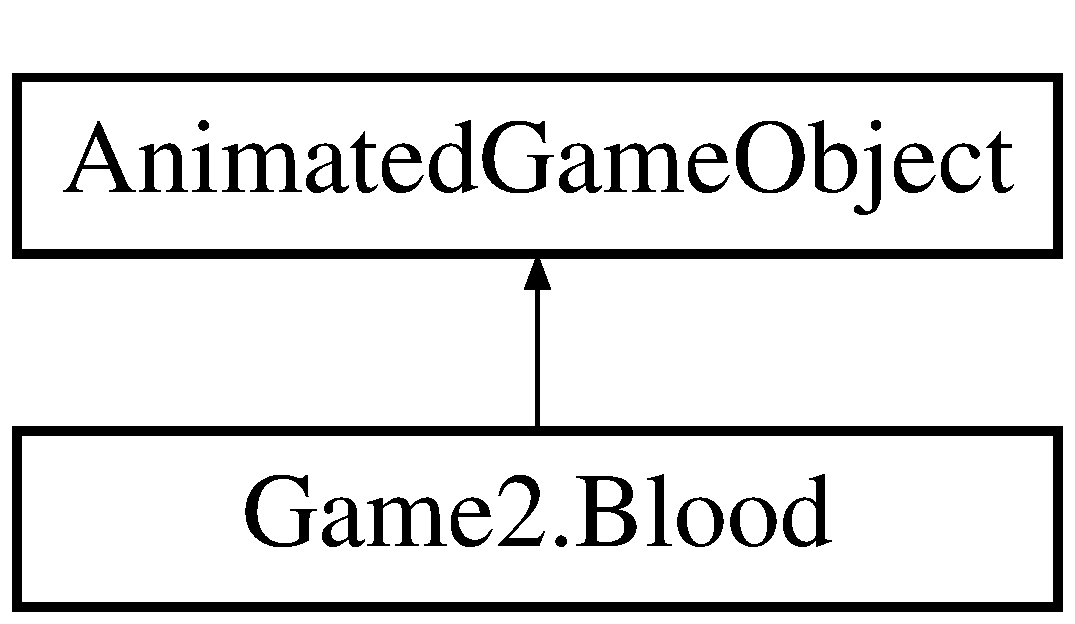
\includegraphics[height=2.000000cm]{class_game2_1_1_blood}
\end{center}
\end{figure}
\subsection*{Public Member Functions}
\begin{DoxyCompactItemize}
\item 
\mbox{\hyperlink{class_game2_1_1_blood_a10ecab2233dc1762d207a443ec1d0e93}{Blood}} (int size, Vector2 start\+Position, Content\+Manager content)
\begin{DoxyCompactList}\small\item\em Adds blood effect when zombies die \end{DoxyCompactList}\item 
override void \mbox{\hyperlink{class_game2_1_1_blood_a3a041247d506eb27de8daafa49daa0cd}{Update}} (Game\+Time game\+Time)
\end{DoxyCompactItemize}


\subsection{Constructor \& Destructor Documentation}
\mbox{\Hypertarget{class_game2_1_1_blood_a10ecab2233dc1762d207a443ec1d0e93}\label{class_game2_1_1_blood_a10ecab2233dc1762d207a443ec1d0e93}} 
\index{Game2\+::\+Blood@{Game2\+::\+Blood}!Blood@{Blood}}
\index{Blood@{Blood}!Game2\+::\+Blood@{Game2\+::\+Blood}}
\subsubsection{\texorpdfstring{Blood()}{Blood()}}
{\footnotesize\ttfamily Game2.\+Blood.\+Blood (\begin{DoxyParamCaption}\item[{int}]{size,  }\item[{Vector2}]{start\+Position,  }\item[{Content\+Manager}]{content }\end{DoxyParamCaption})}



Adds blood effect when zombies die 


\begin{DoxyParams}{Parameters}
{\em size} & \\
\hline
{\em start\+Position} & \\
\hline
{\em content} & \\
\hline
\end{DoxyParams}


\subsection{Member Function Documentation}
\mbox{\Hypertarget{class_game2_1_1_blood_a3a041247d506eb27de8daafa49daa0cd}\label{class_game2_1_1_blood_a3a041247d506eb27de8daafa49daa0cd}} 
\index{Game2\+::\+Blood@{Game2\+::\+Blood}!Update@{Update}}
\index{Update@{Update}!Game2\+::\+Blood@{Game2\+::\+Blood}}
\subsubsection{\texorpdfstring{Update()}{Update()}}
{\footnotesize\ttfamily override void Game2.\+Blood.\+Update (\begin{DoxyParamCaption}\item[{Game\+Time}]{game\+Time }\end{DoxyParamCaption})}



The documentation for this class was generated from the following file\+:\begin{DoxyCompactItemize}
\item 
\mbox{\hyperlink{_blood_8cs}{Blood.\+cs}}\end{DoxyCompactItemize}

\hypertarget{class_game2_1_1_blood_effect}{}\section{Game2.\+Blood\+Effect Class Reference}
\label{class_game2_1_1_blood_effect}\index{Game2.\+Blood\+Effect@{Game2.\+Blood\+Effect}}
Inheritance diagram for Game2.\+Blood\+Effect\+:\begin{figure}[H]
\begin{center}
\leavevmode
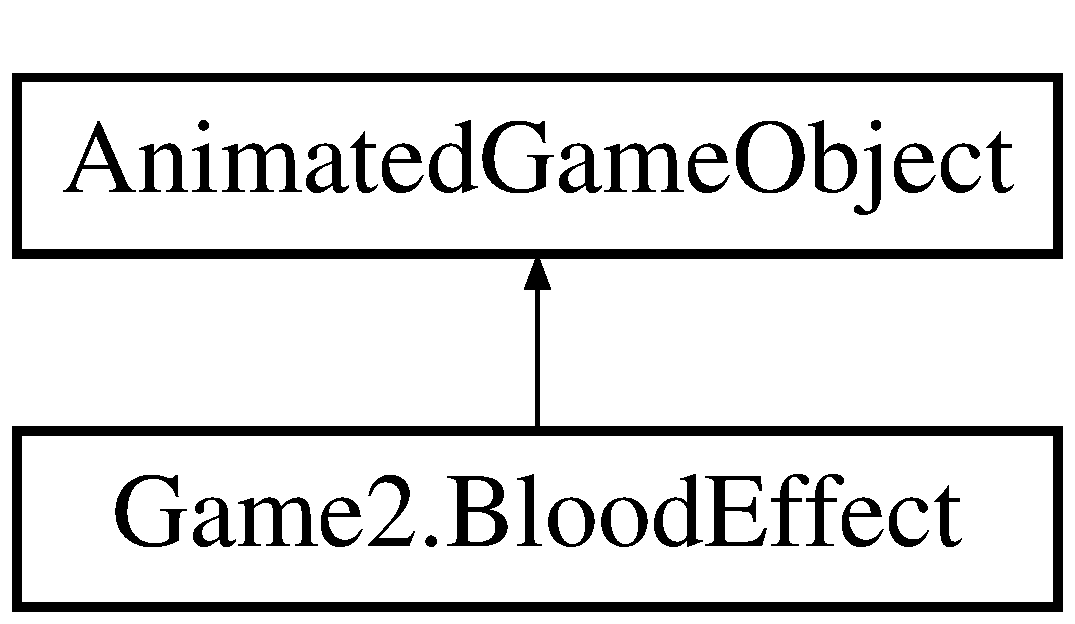
\includegraphics[height=2.000000cm]{class_game2_1_1_blood_effect}
\end{center}
\end{figure}
\subsection*{Public Member Functions}
\begin{DoxyCompactItemize}
\item 
\mbox{\hyperlink{class_game2_1_1_blood_effect_a3d2f1095d0fecc3e822a67128b0bdc46}{Blood\+Effect}} (int size, Vector2 start\+Position, Content\+Manager content)
\begin{DoxyCompactList}\small\item\em Adds blood effect when zombies die \end{DoxyCompactList}\item 
override void \mbox{\hyperlink{class_game2_1_1_blood_effect_a8cde53e26db5632859fb90f87b1dc543}{Update}} (Game\+Time game\+Time)
\end{DoxyCompactItemize}


\subsection{Constructor \& Destructor Documentation}
\mbox{\Hypertarget{class_game2_1_1_blood_effect_a3d2f1095d0fecc3e822a67128b0bdc46}\label{class_game2_1_1_blood_effect_a3d2f1095d0fecc3e822a67128b0bdc46}} 
\index{Game2\+::\+Blood\+Effect@{Game2\+::\+Blood\+Effect}!Blood\+Effect@{Blood\+Effect}}
\index{Blood\+Effect@{Blood\+Effect}!Game2\+::\+Blood\+Effect@{Game2\+::\+Blood\+Effect}}
\subsubsection{\texorpdfstring{Blood\+Effect()}{BloodEffect()}}
{\footnotesize\ttfamily Game2.\+Blood\+Effect.\+Blood\+Effect (\begin{DoxyParamCaption}\item[{int}]{size,  }\item[{Vector2}]{start\+Position,  }\item[{Content\+Manager}]{content }\end{DoxyParamCaption})}



Adds blood effect when zombies die 


\begin{DoxyParams}{Parameters}
{\em size} & \\
\hline
{\em start\+Position} & \\
\hline
{\em content} & \\
\hline
\end{DoxyParams}


\subsection{Member Function Documentation}
\mbox{\Hypertarget{class_game2_1_1_blood_effect_a8cde53e26db5632859fb90f87b1dc543}\label{class_game2_1_1_blood_effect_a8cde53e26db5632859fb90f87b1dc543}} 
\index{Game2\+::\+Blood\+Effect@{Game2\+::\+Blood\+Effect}!Update@{Update}}
\index{Update@{Update}!Game2\+::\+Blood\+Effect@{Game2\+::\+Blood\+Effect}}
\subsubsection{\texorpdfstring{Update()}{Update()}}
{\footnotesize\ttfamily override void Game2.\+Blood\+Effect.\+Update (\begin{DoxyParamCaption}\item[{Game\+Time}]{game\+Time }\end{DoxyParamCaption})}



The documentation for this class was generated from the following file\+:\begin{DoxyCompactItemize}
\item 
Game2/\mbox{\hyperlink{_blood_effect_8cs}{Blood\+Effect.\+cs}}\end{DoxyCompactItemize}

\hypertarget{class_game2_1_1_boss}{}\section{Game2.\+Boss Class Reference}
\label{class_game2_1_1_boss}\index{Game2.\+Boss@{Game2.\+Boss}}


Class that represents a boss  


Inheritance diagram for Game2.\+Boss\+:\begin{figure}[H]
\begin{center}
\leavevmode
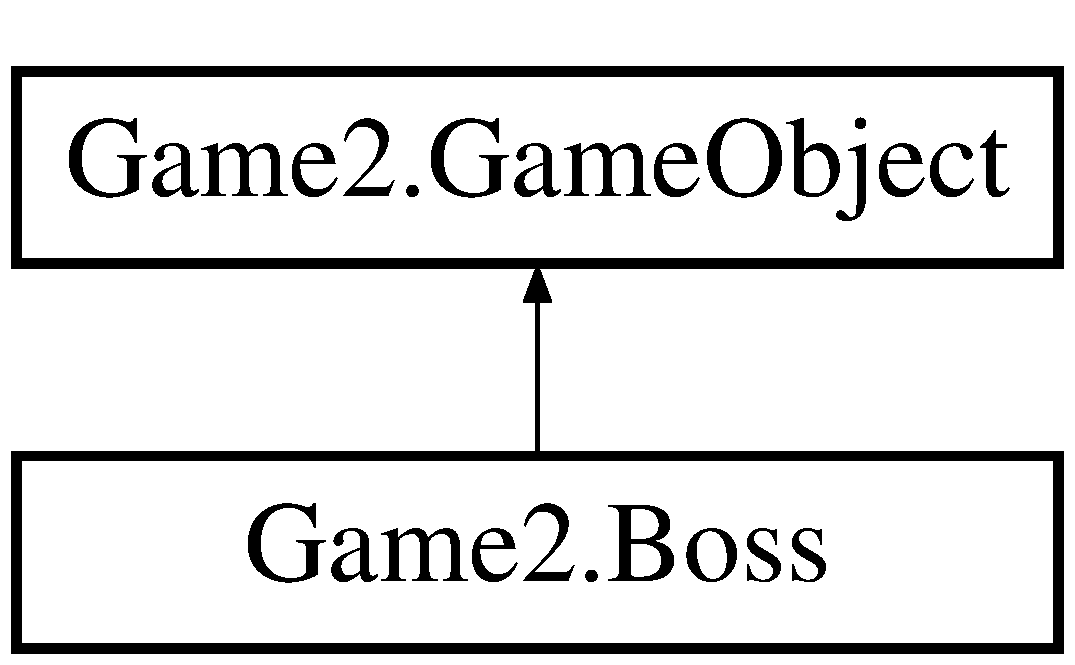
\includegraphics[height=2.000000cm]{class_game2_1_1_boss}
\end{center}
\end{figure}
\subsection*{Public Member Functions}
\begin{DoxyCompactItemize}
\item 
\mbox{\hyperlink{class_game2_1_1_boss_ae7aa8e138bbf3cc4ced004d6ef1f82df}{Boss}} (int Hold\+Number, int Spawn\+Distansfrom\+Each\+Other, Content\+Manager \mbox{\hyperlink{class_game2_1_1_game_object_ae8a9e4574e531d2fbb2168a155f2ac53}{content}})
\begin{DoxyCompactList}\small\item\em Spawns boss at random side of the map \end{DoxyCompactList}\item 
\mbox{\hyperlink{class_game2_1_1_boss_aec980cbbd476cb1b9dde1dd901f5d349}{Boss}} (Content\+Manager \mbox{\hyperlink{class_game2_1_1_game_object_ae8a9e4574e531d2fbb2168a155f2ac53}{content}})
\begin{DoxyCompactList}\small\item\em Spawns boss at random side of the map \end{DoxyCompactList}\item 
override void \mbox{\hyperlink{class_game2_1_1_boss_ab120124b7af0edebcb1664e2feaa6590}{Update}} (Game\+Time game\+Time)
\begin{DoxyCompactList}\small\item\em Update method that moves the boss in direction of the player. \end{DoxyCompactList}\item 
override void \mbox{\hyperlink{class_game2_1_1_boss_a8331b445604b8737664d58bf02f82ce1}{Do\+Collision}} (\mbox{\hyperlink{class_game2_1_1_game_object}{Game\+Object}} other\+Object)
\begin{DoxyCompactList}\small\item\em Collide actions if bullet zombies die and boss loses health. If bullet it gets removed and if player it gets damage. \end{DoxyCompactList}\end{DoxyCompactItemize}
\subsection*{Additional Inherited Members}


\subsection{Detailed Description}
Class that represents a boss 



\subsection{Constructor \& Destructor Documentation}
\mbox{\Hypertarget{class_game2_1_1_boss_ae7aa8e138bbf3cc4ced004d6ef1f82df}\label{class_game2_1_1_boss_ae7aa8e138bbf3cc4ced004d6ef1f82df}} 
\index{Game2\+::\+Boss@{Game2\+::\+Boss}!Boss@{Boss}}
\index{Boss@{Boss}!Game2\+::\+Boss@{Game2\+::\+Boss}}
\subsubsection{\texorpdfstring{Boss()}{Boss()}\hspace{0.1cm}{\footnotesize\ttfamily [1/2]}}
{\footnotesize\ttfamily Game2.\+Boss.\+Boss (\begin{DoxyParamCaption}\item[{int}]{Hold\+Number,  }\item[{int}]{Spawn\+Distansfrom\+Each\+Other,  }\item[{Content\+Manager}]{content }\end{DoxyParamCaption})}



Spawns boss at random side of the map 


\begin{DoxyParams}{Parameters}
{\em content} & Content Manager for loading resources\\
\hline
\end{DoxyParams}
\mbox{\Hypertarget{class_game2_1_1_boss_aec980cbbd476cb1b9dde1dd901f5d349}\label{class_game2_1_1_boss_aec980cbbd476cb1b9dde1dd901f5d349}} 
\index{Game2\+::\+Boss@{Game2\+::\+Boss}!Boss@{Boss}}
\index{Boss@{Boss}!Game2\+::\+Boss@{Game2\+::\+Boss}}
\subsubsection{\texorpdfstring{Boss()}{Boss()}\hspace{0.1cm}{\footnotesize\ttfamily [2/2]}}
{\footnotesize\ttfamily Game2.\+Boss.\+Boss (\begin{DoxyParamCaption}\item[{Content\+Manager}]{content }\end{DoxyParamCaption})}



Spawns boss at random side of the map 


\begin{DoxyParams}{Parameters}
{\em content} & Content Manager for loading resources\\
\hline
\end{DoxyParams}


\subsection{Member Function Documentation}
\mbox{\Hypertarget{class_game2_1_1_boss_a8331b445604b8737664d58bf02f82ce1}\label{class_game2_1_1_boss_a8331b445604b8737664d58bf02f82ce1}} 
\index{Game2\+::\+Boss@{Game2\+::\+Boss}!Do\+Collision@{Do\+Collision}}
\index{Do\+Collision@{Do\+Collision}!Game2\+::\+Boss@{Game2\+::\+Boss}}
\subsubsection{\texorpdfstring{Do\+Collision()}{DoCollision()}}
{\footnotesize\ttfamily override void Game2.\+Boss.\+Do\+Collision (\begin{DoxyParamCaption}\item[{\mbox{\hyperlink{class_game2_1_1_game_object}{Game\+Object}}}]{other\+Object }\end{DoxyParamCaption})\hspace{0.3cm}{\ttfamily [virtual]}}



Collide actions if bullet zombies die and boss loses health. If bullet it gets removed and if player it gets damage. 


\begin{DoxyParams}{Parameters}
{\em other\+Object} & The object it collided with\\
\hline
\end{DoxyParams}


Reimplemented from \mbox{\hyperlink{class_game2_1_1_game_object_aa811d23c405b9aa28ab922901d0a3002}{Game2.\+Game\+Object}}.

\mbox{\Hypertarget{class_game2_1_1_boss_ab120124b7af0edebcb1664e2feaa6590}\label{class_game2_1_1_boss_ab120124b7af0edebcb1664e2feaa6590}} 
\index{Game2\+::\+Boss@{Game2\+::\+Boss}!Update@{Update}}
\index{Update@{Update}!Game2\+::\+Boss@{Game2\+::\+Boss}}
\subsubsection{\texorpdfstring{Update()}{Update()}}
{\footnotesize\ttfamily override void Game2.\+Boss.\+Update (\begin{DoxyParamCaption}\item[{Game\+Time}]{game\+Time }\end{DoxyParamCaption})\hspace{0.3cm}{\ttfamily [virtual]}}



Update method that moves the boss in direction of the player. 


\begin{DoxyParams}{Parameters}
{\em game\+Time} & \\
\hline
\end{DoxyParams}


Reimplemented from \mbox{\hyperlink{class_game2_1_1_game_object_a360a294d8a55dcc747c44f8cc1aefe28}{Game2.\+Game\+Object}}.



The documentation for this class was generated from the following file\+:\begin{DoxyCompactItemize}
\item 
Game2/\mbox{\hyperlink{_boss_8cs}{Boss.\+cs}}\end{DoxyCompactItemize}

\hypertarget{class_game2_1_1_bullet}{}\section{Game2.\+Bullet Class Reference}
\label{class_game2_1_1_bullet}\index{Game2.\+Bullet@{Game2.\+Bullet}}


Class that represents a \mbox{\hyperlink{class_game2_1_1_bullet}{Bullet}} fired from the player  


Inheritance diagram for Game2.\+Bullet\+:\begin{figure}[H]
\begin{center}
\leavevmode
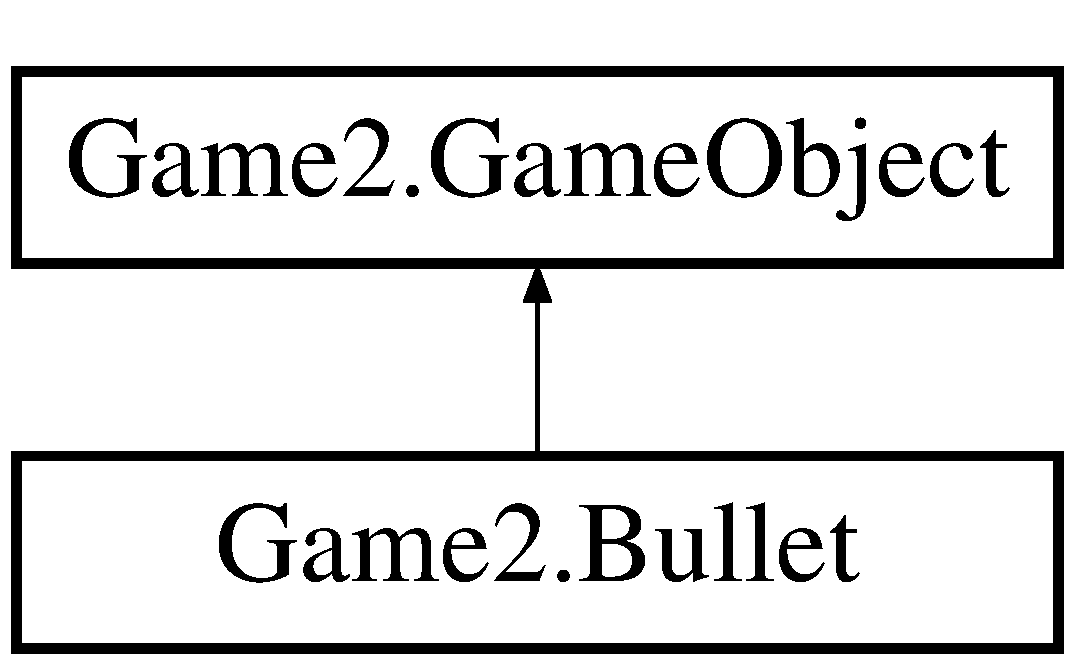
\includegraphics[height=2.000000cm]{class_game2_1_1_bullet}
\end{center}
\end{figure}
\subsection*{Public Member Functions}
\begin{DoxyCompactItemize}
\item 
\mbox{\hyperlink{class_game2_1_1_bullet_aa5376505fe806d88f708315e7ecdacb6}{Bullet}} (Vector2 direction, Vector2 start\+Position, Content\+Manager \mbox{\hyperlink{class_game2_1_1_game_object_ae8a9e4574e531d2fbb2168a155f2ac53}{content}})
\begin{DoxyCompactList}\small\item\em Constructor for a \mbox{\hyperlink{class_game2_1_1_bullet}{Bullet}} \end{DoxyCompactList}\item 
override void \mbox{\hyperlink{class_game2_1_1_bullet_a2cf7c4b1a587f2b7e92611d5f6173d3e}{Update}} (Game\+Time game\+Time)
\begin{DoxyCompactList}\small\item\em Moves the \mbox{\hyperlink{class_game2_1_1_bullet}{Bullet}} in the designated direction. If it goes outside the screen area it gets removed \end{DoxyCompactList}\end{DoxyCompactItemize}
\subsection*{Additional Inherited Members}


\subsection{Detailed Description}
Class that represents a \mbox{\hyperlink{class_game2_1_1_bullet}{Bullet}} fired from the player 



\subsection{Constructor \& Destructor Documentation}
\mbox{\Hypertarget{class_game2_1_1_bullet_aa5376505fe806d88f708315e7ecdacb6}\label{class_game2_1_1_bullet_aa5376505fe806d88f708315e7ecdacb6}} 
\index{Game2\+::\+Bullet@{Game2\+::\+Bullet}!Bullet@{Bullet}}
\index{Bullet@{Bullet}!Game2\+::\+Bullet@{Game2\+::\+Bullet}}
\subsubsection{\texorpdfstring{Bullet()}{Bullet()}}
{\footnotesize\ttfamily Game2.\+Bullet.\+Bullet (\begin{DoxyParamCaption}\item[{Vector2}]{direction,  }\item[{Vector2}]{start\+Position,  }\item[{Content\+Manager}]{content }\end{DoxyParamCaption})}



Constructor for a \mbox{\hyperlink{class_game2_1_1_bullet}{Bullet}} 


\begin{DoxyParams}{Parameters}
{\em direction} & Sets the movement direction for the \mbox{\hyperlink{class_game2_1_1_bullet}{Bullet}}\\
\hline
{\em start\+Position} & Sets its starting position\\
\hline
{\em content} & Content Manager for loading resources\\
\hline
\end{DoxyParams}


\subsection{Member Function Documentation}
\mbox{\Hypertarget{class_game2_1_1_bullet_a2cf7c4b1a587f2b7e92611d5f6173d3e}\label{class_game2_1_1_bullet_a2cf7c4b1a587f2b7e92611d5f6173d3e}} 
\index{Game2\+::\+Bullet@{Game2\+::\+Bullet}!Update@{Update}}
\index{Update@{Update}!Game2\+::\+Bullet@{Game2\+::\+Bullet}}
\subsubsection{\texorpdfstring{Update()}{Update()}}
{\footnotesize\ttfamily override void Game2.\+Bullet.\+Update (\begin{DoxyParamCaption}\item[{Game\+Time}]{game\+Time }\end{DoxyParamCaption})\hspace{0.3cm}{\ttfamily [virtual]}}



Moves the \mbox{\hyperlink{class_game2_1_1_bullet}{Bullet}} in the designated direction. If it goes outside the screen area it gets removed 


\begin{DoxyParams}{Parameters}
{\em game\+Time} & The elasped time since last update call\\
\hline
\end{DoxyParams}


Reimplemented from \mbox{\hyperlink{class_game2_1_1_game_object_a360a294d8a55dcc747c44f8cc1aefe28}{Game2.\+Game\+Object}}.



The documentation for this class was generated from the following file\+:\begin{DoxyCompactItemize}
\item 
Game2/\mbox{\hyperlink{_bullet_8cs}{Bullet.\+cs}}\end{DoxyCompactItemize}

\hypertarget{class_game2_1_1_enemy}{}\section{Game2.\+Enemy Class Reference}
\label{class_game2_1_1_enemy}\index{Game2.\+Enemy@{Game2.\+Enemy}}


Class that represents a zombie  


Inheritance diagram for Game2.\+Enemy\+:\begin{figure}[H]
\begin{center}
\leavevmode
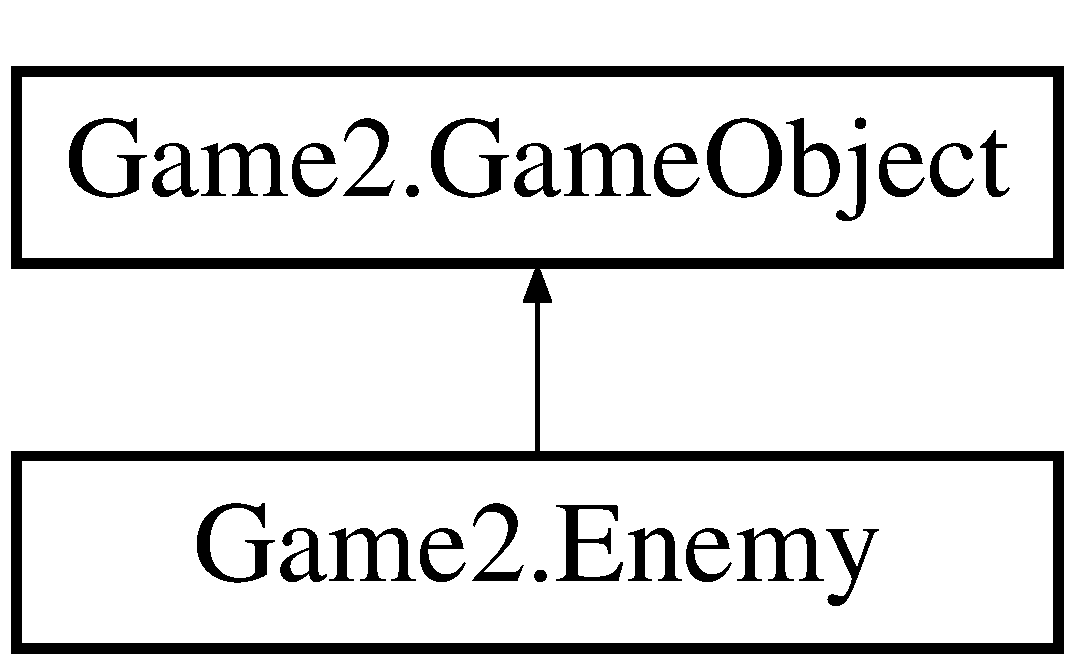
\includegraphics[height=2.000000cm]{class_game2_1_1_enemy}
\end{center}
\end{figure}
\subsection*{Public Member Functions}
\begin{DoxyCompactItemize}
\item 
\mbox{\hyperlink{class_game2_1_1_enemy_ac96eace4797abdd8d99c0e67348f1f7d}{Enemy}} (int Hold\+Number, int Spawn\+Distansfrom\+Each\+Other, Content\+Manager \mbox{\hyperlink{class_game2_1_1_game_object_ae8a9e4574e531d2fbb2168a155f2ac53}{content}})
\begin{DoxyCompactList}\small\item\em Spawns zombies at random sides of the map \end{DoxyCompactList}\item 
\mbox{\hyperlink{class_game2_1_1_enemy_abb82db1812e2fa2b074f0bc0c53471d1}{Enemy}} (Content\+Manager \mbox{\hyperlink{class_game2_1_1_game_object_ae8a9e4574e531d2fbb2168a155f2ac53}{content}})
\begin{DoxyCompactList}\small\item\em Spawns zombies at random sides of the map \end{DoxyCompactList}\item 
override void \mbox{\hyperlink{class_game2_1_1_enemy_a5e3fdb40fb9884bda064eb671896d264}{Update}} (Game\+Time game\+Time)
\begin{DoxyCompactList}\small\item\em Update method that moves the zombies in direction of the player. \end{DoxyCompactList}\item 
override void \mbox{\hyperlink{class_game2_1_1_enemy_a574b0e99f86ce3a5e126484518020dac}{Do\+Collision}} (\mbox{\hyperlink{class_game2_1_1_game_object}{Game\+Object}} other\+Object)
\begin{DoxyCompactList}\small\item\em Collide actions if bullet zombies die and boss loses health. If bullet it gets removed and if player it gets damage. \end{DoxyCompactList}\end{DoxyCompactItemize}
\subsection*{Additional Inherited Members}


\subsection{Detailed Description}
Class that represents a zombie 



\subsection{Constructor \& Destructor Documentation}
\mbox{\Hypertarget{class_game2_1_1_enemy_ac96eace4797abdd8d99c0e67348f1f7d}\label{class_game2_1_1_enemy_ac96eace4797abdd8d99c0e67348f1f7d}} 
\index{Game2\+::\+Enemy@{Game2\+::\+Enemy}!Enemy@{Enemy}}
\index{Enemy@{Enemy}!Game2\+::\+Enemy@{Game2\+::\+Enemy}}
\subsubsection{\texorpdfstring{Enemy()}{Enemy()}\hspace{0.1cm}{\footnotesize\ttfamily [1/2]}}
{\footnotesize\ttfamily Game2.\+Enemy.\+Enemy (\begin{DoxyParamCaption}\item[{int}]{Hold\+Number,  }\item[{int}]{Spawn\+Distansfrom\+Each\+Other,  }\item[{Content\+Manager}]{content }\end{DoxyParamCaption})}



Spawns zombies at random sides of the map 


\begin{DoxyParams}{Parameters}
{\em content} & Content Manager for loading resources\\
\hline
\end{DoxyParams}
\mbox{\Hypertarget{class_game2_1_1_enemy_abb82db1812e2fa2b074f0bc0c53471d1}\label{class_game2_1_1_enemy_abb82db1812e2fa2b074f0bc0c53471d1}} 
\index{Game2\+::\+Enemy@{Game2\+::\+Enemy}!Enemy@{Enemy}}
\index{Enemy@{Enemy}!Game2\+::\+Enemy@{Game2\+::\+Enemy}}
\subsubsection{\texorpdfstring{Enemy()}{Enemy()}\hspace{0.1cm}{\footnotesize\ttfamily [2/2]}}
{\footnotesize\ttfamily Game2.\+Enemy.\+Enemy (\begin{DoxyParamCaption}\item[{Content\+Manager}]{content }\end{DoxyParamCaption})}



Spawns zombies at random sides of the map 


\begin{DoxyParams}{Parameters}
{\em content} & Content Manager for loading resources\\
\hline
\end{DoxyParams}


\subsection{Member Function Documentation}
\mbox{\Hypertarget{class_game2_1_1_enemy_a574b0e99f86ce3a5e126484518020dac}\label{class_game2_1_1_enemy_a574b0e99f86ce3a5e126484518020dac}} 
\index{Game2\+::\+Enemy@{Game2\+::\+Enemy}!Do\+Collision@{Do\+Collision}}
\index{Do\+Collision@{Do\+Collision}!Game2\+::\+Enemy@{Game2\+::\+Enemy}}
\subsubsection{\texorpdfstring{Do\+Collision()}{DoCollision()}}
{\footnotesize\ttfamily override void Game2.\+Enemy.\+Do\+Collision (\begin{DoxyParamCaption}\item[{\mbox{\hyperlink{class_game2_1_1_game_object}{Game\+Object}}}]{other\+Object }\end{DoxyParamCaption})\hspace{0.3cm}{\ttfamily [virtual]}}



Collide actions if bullet zombies die and boss loses health. If bullet it gets removed and if player it gets damage. 


\begin{DoxyParams}{Parameters}
{\em other\+Object} & The object it collided with\\
\hline
\end{DoxyParams}


Reimplemented from \mbox{\hyperlink{class_game2_1_1_game_object_aa811d23c405b9aa28ab922901d0a3002}{Game2.\+Game\+Object}}.

\mbox{\Hypertarget{class_game2_1_1_enemy_a5e3fdb40fb9884bda064eb671896d264}\label{class_game2_1_1_enemy_a5e3fdb40fb9884bda064eb671896d264}} 
\index{Game2\+::\+Enemy@{Game2\+::\+Enemy}!Update@{Update}}
\index{Update@{Update}!Game2\+::\+Enemy@{Game2\+::\+Enemy}}
\subsubsection{\texorpdfstring{Update()}{Update()}}
{\footnotesize\ttfamily override void Game2.\+Enemy.\+Update (\begin{DoxyParamCaption}\item[{Game\+Time}]{game\+Time }\end{DoxyParamCaption})\hspace{0.3cm}{\ttfamily [virtual]}}



Update method that moves the zombies in direction of the player. 


\begin{DoxyParams}{Parameters}
{\em game\+Time} & \\
\hline
\end{DoxyParams}


Reimplemented from \mbox{\hyperlink{class_game2_1_1_game_object_a360a294d8a55dcc747c44f8cc1aefe28}{Game2.\+Game\+Object}}.



The documentation for this class was generated from the following file\+:\begin{DoxyCompactItemize}
\item 
\mbox{\hyperlink{_enemy_8cs}{Enemy.\+cs}}\end{DoxyCompactItemize}

\hypertarget{class_game2_1_1_game_object}{}\section{Game2.\+Game\+Object Class Reference}
\label{class_game2_1_1_game_object}\index{Game2.\+Game\+Object@{Game2.\+Game\+Object}}
Inheritance diagram for Game2.\+Game\+Object\+:\begin{figure}[H]
\begin{center}
\leavevmode
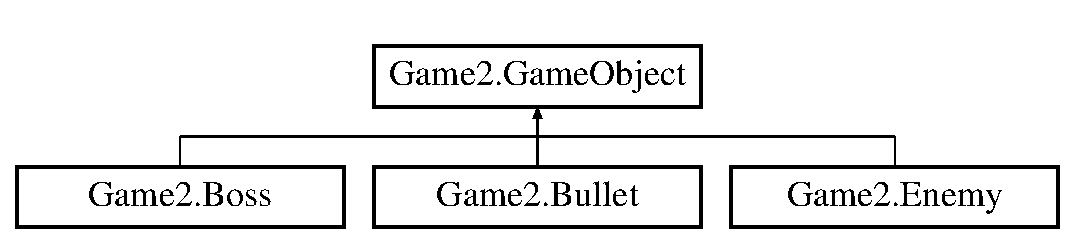
\includegraphics[height=2.000000cm]{class_game2_1_1_game_object}
\end{center}
\end{figure}
\subsection*{Public Member Functions}
\begin{DoxyCompactItemize}
\item 
bool \mbox{\hyperlink{class_game2_1_1_game_object_a043206229a679b32a1bee4f50e8e7ace}{Is\+Colliding}} (\mbox{\hyperlink{class_game2_1_1_game_object}{Game\+Object}} other\+Object)
\begin{DoxyCompactList}\small\item\em Checks if the current object collides with another object \end{DoxyCompactList}\item 
virtual void \mbox{\hyperlink{class_game2_1_1_game_object_aa811d23c405b9aa28ab922901d0a3002}{Do\+Collision}} (\mbox{\hyperlink{class_game2_1_1_game_object}{Game\+Object}} other\+Object)
\begin{DoxyCompactList}\small\item\em Enabled the \mbox{\hyperlink{class_game2_1_1_game_object}{Game\+Object}} to handle collisions in a custom way \end{DoxyCompactList}\item 
\mbox{\hyperlink{class_game2_1_1_game_object_ad2a99e120df1d04d1a737bbf9b8fb2a0}{Game\+Object}} (Content\+Manager \mbox{\hyperlink{class_game2_1_1_game_object_ae8a9e4574e531d2fbb2168a155f2ac53}{content}}, string sprite\+Name)
\begin{DoxyCompactList}\small\item\em The default constructor for a \mbox{\hyperlink{class_game2_1_1_game_object}{Game\+Object}} \end{DoxyCompactList}\item 
void \mbox{\hyperlink{class_game2_1_1_game_object_a3379bff2fa0d79ae4eeea4f1e9609064}{Get\+Player\+Position}} (Vector2 Player\+Position)
\begin{DoxyCompactList}\small\item\em Gets the position and rotaion of player \end{DoxyCompactList}\item 
void \mbox{\hyperlink{class_game2_1_1_game_object_aae6ebb6727aabac812b8bcc68aba2484}{Get\+Player\+Rot}} (float Player\+Rot)
\item 
void \mbox{\hyperlink{class_game2_1_1_game_object_add937595f4f6918a828af495c08bce3d}{Get\+Player\+Health}} (int player\+Heath)
\item 
int \mbox{\hyperlink{class_game2_1_1_game_object_a9db72e4b451539bf698e5e1dcd6e12c4}{return\+Player\+Health}} ()
\item 
\mbox{\hyperlink{class_game2_1_1_game_object_a52d0c63362ab13bf5d0433c42b9b4ffb}{Game\+Object}} (Vector2 start\+Position, Content\+Manager \mbox{\hyperlink{class_game2_1_1_game_object_ae8a9e4574e531d2fbb2168a155f2ac53}{content}}, string sprite\+Name)
\begin{DoxyCompactList}\small\item\em Constructor the sets the staring position of the \mbox{\hyperlink{class_game2_1_1_game_object}{Game\+Object}} \end{DoxyCompactList}\item 
virtual void \mbox{\hyperlink{class_game2_1_1_game_object_a360a294d8a55dcc747c44f8cc1aefe28}{Update}} (Game\+Time game\+Time)
\begin{DoxyCompactList}\small\item\em Enabled the \mbox{\hyperlink{class_game2_1_1_game_object}{Game\+Object}} to have game logic defined \end{DoxyCompactList}\item 
virtual void \mbox{\hyperlink{class_game2_1_1_game_object_ade17d36d8d908594bc434e215052393b}{Draw}} (Sprite\+Batch sprite\+Batch)
\begin{DoxyCompactList}\small\item\em Enables the \mbox{\hyperlink{class_game2_1_1_game_object}{Game\+Object}} to be drawn. The std. functionality is to draw its sprite. \end{DoxyCompactList}\end{DoxyCompactItemize}
\subsection*{Protected Attributes}
\begin{DoxyCompactItemize}
\item 
Texture2D \mbox{\hyperlink{class_game2_1_1_game_object_abd502421a8463bab3dc736266be6de26}{sprite}}
\item 
float \mbox{\hyperlink{class_game2_1_1_game_object_a97359c68fe62861ff5ad578130367493}{rotation}}
\item 
Vector2 \mbox{\hyperlink{class_game2_1_1_game_object_a5bc3b9c88ad0ce089558862431923192}{Direction}}
\item 
Vector2 \mbox{\hyperlink{class_game2_1_1_game_object_a1564c00bda65516c2486548dda1cbc1c}{position}}
\item 
Vector2 \mbox{\hyperlink{class_game2_1_1_game_object_a8e9bcc1b5d686ef1a49337744fb3c0c1}{real\+Timeplayer\+Position}}
\item 
float \mbox{\hyperlink{class_game2_1_1_game_object_a8103636301612d46cbfaf40a295cf889}{real\+Timeplayer\+Rot}}
\item 
int \mbox{\hyperlink{class_game2_1_1_game_object_a58bb9938314474563d84b283ab651178}{Playerhealth}}
\item 
int \mbox{\hyperlink{class_game2_1_1_game_object_a983dc42585d2eefbc27bd59a2e39a467}{la}} = 700
\item 
Content\+Manager \mbox{\hyperlink{class_game2_1_1_game_object_ae8a9e4574e531d2fbb2168a155f2ac53}{content}}
\end{DoxyCompactItemize}
\subsection*{Properties}
\begin{DoxyCompactItemize}
\item 
Vector2 \mbox{\hyperlink{class_game2_1_1_game_object_af5b0b48192336247e09d52a7fc6f56ad}{Position}}\hspace{0.3cm}{\ttfamily  \mbox{[}get\mbox{]}}
\item 
float \mbox{\hyperlink{class_game2_1_1_game_object_a7983716d3a4ed64a1a2200642a301079}{player\+Rot}}\hspace{0.3cm}{\ttfamily  \mbox{[}get\mbox{]}}
\item 
virtual Rectangle \mbox{\hyperlink{class_game2_1_1_game_object_ab6a6d45b66a978f710da6a3ec0588083}{Collision\+Box}}\hspace{0.3cm}{\ttfamily  \mbox{[}get\mbox{]}}
\begin{DoxyCompactList}\small\item\em The Collision Box of the \mbox{\hyperlink{class_game2_1_1_game_object}{Game\+Object}}. The default box is based upon the \mbox{\hyperlink{class_game2_1_1_game_object}{Game\+Object}} position and sprite size \end{DoxyCompactList}\end{DoxyCompactItemize}


\subsection{Constructor \& Destructor Documentation}
\mbox{\Hypertarget{class_game2_1_1_game_object_ad2a99e120df1d04d1a737bbf9b8fb2a0}\label{class_game2_1_1_game_object_ad2a99e120df1d04d1a737bbf9b8fb2a0}} 
\index{Game2\+::\+Game\+Object@{Game2\+::\+Game\+Object}!Game\+Object@{Game\+Object}}
\index{Game\+Object@{Game\+Object}!Game2\+::\+Game\+Object@{Game2\+::\+Game\+Object}}
\subsubsection{\texorpdfstring{Game\+Object()}{GameObject()}\hspace{0.1cm}{\footnotesize\ttfamily [1/2]}}
{\footnotesize\ttfamily Game2.\+Game\+Object.\+Game\+Object (\begin{DoxyParamCaption}\item[{Content\+Manager}]{content,  }\item[{string}]{sprite\+Name }\end{DoxyParamCaption})}



The default constructor for a \mbox{\hyperlink{class_game2_1_1_game_object}{Game\+Object}} 


\begin{DoxyParams}{Parameters}
{\em content} & Reference to a Content\+Manager for loading resources\\
\hline
{\em sprite\+Name} & The name of the texture resource the should be used for the sprite\\
\hline
\end{DoxyParams}

\begin{DoxyExceptions}{Exceptions}
{\em Microsoft.\+Xna.\+Framework.\+Content.\+Content\+Load\+Exception} & Thrown if a matching texture cant be found for sprite\+Name\\
\hline
\end{DoxyExceptions}
\mbox{\Hypertarget{class_game2_1_1_game_object_a52d0c63362ab13bf5d0433c42b9b4ffb}\label{class_game2_1_1_game_object_a52d0c63362ab13bf5d0433c42b9b4ffb}} 
\index{Game2\+::\+Game\+Object@{Game2\+::\+Game\+Object}!Game\+Object@{Game\+Object}}
\index{Game\+Object@{Game\+Object}!Game2\+::\+Game\+Object@{Game2\+::\+Game\+Object}}
\subsubsection{\texorpdfstring{Game\+Object()}{GameObject()}\hspace{0.1cm}{\footnotesize\ttfamily [2/2]}}
{\footnotesize\ttfamily Game2.\+Game\+Object.\+Game\+Object (\begin{DoxyParamCaption}\item[{Vector2}]{start\+Position,  }\item[{Content\+Manager}]{content,  }\item[{string}]{sprite\+Name }\end{DoxyParamCaption})}



Constructor the sets the staring position of the \mbox{\hyperlink{class_game2_1_1_game_object}{Game\+Object}} 


\begin{DoxyParams}{Parameters}
{\em start\+Position} & \\
\hline
{\em content} & Reference to a Content\+Manager for loading resources\\
\hline
{\em sprite\+Name} & The name of the texture resource the should be used for the sprite\\
\hline
\end{DoxyParams}

\begin{DoxyExceptions}{Exceptions}
{\em Microsoft.\+Xna.\+Framework.\+Content.\+Content\+Load\+Exception} & Thrown if a matching texture cant be found for sprite\+Name\\
\hline
\end{DoxyExceptions}


\subsection{Member Function Documentation}
\mbox{\Hypertarget{class_game2_1_1_game_object_aa811d23c405b9aa28ab922901d0a3002}\label{class_game2_1_1_game_object_aa811d23c405b9aa28ab922901d0a3002}} 
\index{Game2\+::\+Game\+Object@{Game2\+::\+Game\+Object}!Do\+Collision@{Do\+Collision}}
\index{Do\+Collision@{Do\+Collision}!Game2\+::\+Game\+Object@{Game2\+::\+Game\+Object}}
\subsubsection{\texorpdfstring{Do\+Collision()}{DoCollision()}}
{\footnotesize\ttfamily virtual void Game2.\+Game\+Object.\+Do\+Collision (\begin{DoxyParamCaption}\item[{\mbox{\hyperlink{class_game2_1_1_game_object}{Game\+Object}}}]{other\+Object }\end{DoxyParamCaption})\hspace{0.3cm}{\ttfamily [virtual]}}



Enabled the \mbox{\hyperlink{class_game2_1_1_game_object}{Game\+Object}} to handle collisions in a custom way 


\begin{DoxyParams}{Parameters}
{\em other\+Object} & The \mbox{\hyperlink{class_game2_1_1_game_object}{Game\+Object}} that the current \mbox{\hyperlink{class_game2_1_1_game_object}{Game\+Object}} collides with\\
\hline
\end{DoxyParams}


Reimplemented in \mbox{\hyperlink{class_game2_1_1_boss_a8331b445604b8737664d58bf02f82ce1}{Game2.\+Boss}}, and \mbox{\hyperlink{class_game2_1_1_enemy_a574b0e99f86ce3a5e126484518020dac}{Game2.\+Enemy}}.

\mbox{\Hypertarget{class_game2_1_1_game_object_ade17d36d8d908594bc434e215052393b}\label{class_game2_1_1_game_object_ade17d36d8d908594bc434e215052393b}} 
\index{Game2\+::\+Game\+Object@{Game2\+::\+Game\+Object}!Draw@{Draw}}
\index{Draw@{Draw}!Game2\+::\+Game\+Object@{Game2\+::\+Game\+Object}}
\subsubsection{\texorpdfstring{Draw()}{Draw()}}
{\footnotesize\ttfamily virtual void Game2.\+Game\+Object.\+Draw (\begin{DoxyParamCaption}\item[{Sprite\+Batch}]{sprite\+Batch }\end{DoxyParamCaption})\hspace{0.3cm}{\ttfamily [virtual]}}



Enables the \mbox{\hyperlink{class_game2_1_1_game_object}{Game\+Object}} to be drawn. The std. functionality is to draw its sprite. 


\begin{DoxyParams}{Parameters}
{\em sprite\+Batch} & The spritebatch to use for drawing\\
\hline
\end{DoxyParams}
\mbox{\Hypertarget{class_game2_1_1_game_object_add937595f4f6918a828af495c08bce3d}\label{class_game2_1_1_game_object_add937595f4f6918a828af495c08bce3d}} 
\index{Game2\+::\+Game\+Object@{Game2\+::\+Game\+Object}!Get\+Player\+Health@{Get\+Player\+Health}}
\index{Get\+Player\+Health@{Get\+Player\+Health}!Game2\+::\+Game\+Object@{Game2\+::\+Game\+Object}}
\subsubsection{\texorpdfstring{Get\+Player\+Health()}{GetPlayerHealth()}}
{\footnotesize\ttfamily void Game2.\+Game\+Object.\+Get\+Player\+Health (\begin{DoxyParamCaption}\item[{int}]{player\+Heath }\end{DoxyParamCaption})}

\mbox{\Hypertarget{class_game2_1_1_game_object_a3379bff2fa0d79ae4eeea4f1e9609064}\label{class_game2_1_1_game_object_a3379bff2fa0d79ae4eeea4f1e9609064}} 
\index{Game2\+::\+Game\+Object@{Game2\+::\+Game\+Object}!Get\+Player\+Position@{Get\+Player\+Position}}
\index{Get\+Player\+Position@{Get\+Player\+Position}!Game2\+::\+Game\+Object@{Game2\+::\+Game\+Object}}
\subsubsection{\texorpdfstring{Get\+Player\+Position()}{GetPlayerPosition()}}
{\footnotesize\ttfamily void Game2.\+Game\+Object.\+Get\+Player\+Position (\begin{DoxyParamCaption}\item[{Vector2}]{Player\+Position }\end{DoxyParamCaption})}



Gets the position and rotaion of player 


\begin{DoxyParams}{Parameters}
{\em Player\+Position} & \\
\hline
\end{DoxyParams}
\mbox{\Hypertarget{class_game2_1_1_game_object_aae6ebb6727aabac812b8bcc68aba2484}\label{class_game2_1_1_game_object_aae6ebb6727aabac812b8bcc68aba2484}} 
\index{Game2\+::\+Game\+Object@{Game2\+::\+Game\+Object}!Get\+Player\+Rot@{Get\+Player\+Rot}}
\index{Get\+Player\+Rot@{Get\+Player\+Rot}!Game2\+::\+Game\+Object@{Game2\+::\+Game\+Object}}
\subsubsection{\texorpdfstring{Get\+Player\+Rot()}{GetPlayerRot()}}
{\footnotesize\ttfamily void Game2.\+Game\+Object.\+Get\+Player\+Rot (\begin{DoxyParamCaption}\item[{float}]{Player\+Rot }\end{DoxyParamCaption})}

\mbox{\Hypertarget{class_game2_1_1_game_object_a043206229a679b32a1bee4f50e8e7ace}\label{class_game2_1_1_game_object_a043206229a679b32a1bee4f50e8e7ace}} 
\index{Game2\+::\+Game\+Object@{Game2\+::\+Game\+Object}!Is\+Colliding@{Is\+Colliding}}
\index{Is\+Colliding@{Is\+Colliding}!Game2\+::\+Game\+Object@{Game2\+::\+Game\+Object}}
\subsubsection{\texorpdfstring{Is\+Colliding()}{IsColliding()}}
{\footnotesize\ttfamily bool Game2.\+Game\+Object.\+Is\+Colliding (\begin{DoxyParamCaption}\item[{\mbox{\hyperlink{class_game2_1_1_game_object}{Game\+Object}}}]{other\+Object }\end{DoxyParamCaption})}



Checks if the current object collides with another object 


\begin{DoxyParams}{Parameters}
{\em other\+Object} & The other \mbox{\hyperlink{class_game2_1_1_game_object}{Game\+Object}} that should be tested against\\
\hline
\end{DoxyParams}
\begin{DoxyReturn}{Returns}
Returns true if current object collides with other\+Object otherwise false
\end{DoxyReturn}
\mbox{\Hypertarget{class_game2_1_1_game_object_a9db72e4b451539bf698e5e1dcd6e12c4}\label{class_game2_1_1_game_object_a9db72e4b451539bf698e5e1dcd6e12c4}} 
\index{Game2\+::\+Game\+Object@{Game2\+::\+Game\+Object}!return\+Player\+Health@{return\+Player\+Health}}
\index{return\+Player\+Health@{return\+Player\+Health}!Game2\+::\+Game\+Object@{Game2\+::\+Game\+Object}}
\subsubsection{\texorpdfstring{return\+Player\+Health()}{returnPlayerHealth()}}
{\footnotesize\ttfamily int Game2.\+Game\+Object.\+return\+Player\+Health (\begin{DoxyParamCaption}{ }\end{DoxyParamCaption})}

\mbox{\Hypertarget{class_game2_1_1_game_object_a360a294d8a55dcc747c44f8cc1aefe28}\label{class_game2_1_1_game_object_a360a294d8a55dcc747c44f8cc1aefe28}} 
\index{Game2\+::\+Game\+Object@{Game2\+::\+Game\+Object}!Update@{Update}}
\index{Update@{Update}!Game2\+::\+Game\+Object@{Game2\+::\+Game\+Object}}
\subsubsection{\texorpdfstring{Update()}{Update()}}
{\footnotesize\ttfamily virtual void Game2.\+Game\+Object.\+Update (\begin{DoxyParamCaption}\item[{Game\+Time}]{game\+Time }\end{DoxyParamCaption})\hspace{0.3cm}{\ttfamily [virtual]}}



Enabled the \mbox{\hyperlink{class_game2_1_1_game_object}{Game\+Object}} to have game logic defined 


\begin{DoxyParams}{Parameters}
{\em game\+Time} & The elasped time since last update call\\
\hline
\end{DoxyParams}


Reimplemented in \mbox{\hyperlink{class_game2_1_1_boss_ab120124b7af0edebcb1664e2feaa6590}{Game2.\+Boss}}, \mbox{\hyperlink{class_game2_1_1_enemy_a5e3fdb40fb9884bda064eb671896d264}{Game2.\+Enemy}}, and \mbox{\hyperlink{class_game2_1_1_bullet_a2cf7c4b1a587f2b7e92611d5f6173d3e}{Game2.\+Bullet}}.



\subsection{Member Data Documentation}
\mbox{\Hypertarget{class_game2_1_1_game_object_ae8a9e4574e531d2fbb2168a155f2ac53}\label{class_game2_1_1_game_object_ae8a9e4574e531d2fbb2168a155f2ac53}} 
\index{Game2\+::\+Game\+Object@{Game2\+::\+Game\+Object}!content@{content}}
\index{content@{content}!Game2\+::\+Game\+Object@{Game2\+::\+Game\+Object}}
\subsubsection{\texorpdfstring{content}{content}}
{\footnotesize\ttfamily Content\+Manager Game2.\+Game\+Object.\+content\hspace{0.3cm}{\ttfamily [protected]}}

\mbox{\Hypertarget{class_game2_1_1_game_object_a5bc3b9c88ad0ce089558862431923192}\label{class_game2_1_1_game_object_a5bc3b9c88ad0ce089558862431923192}} 
\index{Game2\+::\+Game\+Object@{Game2\+::\+Game\+Object}!Direction@{Direction}}
\index{Direction@{Direction}!Game2\+::\+Game\+Object@{Game2\+::\+Game\+Object}}
\subsubsection{\texorpdfstring{Direction}{Direction}}
{\footnotesize\ttfamily Vector2 Game2.\+Game\+Object.\+Direction\hspace{0.3cm}{\ttfamily [protected]}}

\mbox{\Hypertarget{class_game2_1_1_game_object_a983dc42585d2eefbc27bd59a2e39a467}\label{class_game2_1_1_game_object_a983dc42585d2eefbc27bd59a2e39a467}} 
\index{Game2\+::\+Game\+Object@{Game2\+::\+Game\+Object}!la@{la}}
\index{la@{la}!Game2\+::\+Game\+Object@{Game2\+::\+Game\+Object}}
\subsubsection{\texorpdfstring{la}{la}}
{\footnotesize\ttfamily int Game2.\+Game\+Object.\+la = 700\hspace{0.3cm}{\ttfamily [protected]}}

\mbox{\Hypertarget{class_game2_1_1_game_object_a58bb9938314474563d84b283ab651178}\label{class_game2_1_1_game_object_a58bb9938314474563d84b283ab651178}} 
\index{Game2\+::\+Game\+Object@{Game2\+::\+Game\+Object}!Playerhealth@{Playerhealth}}
\index{Playerhealth@{Playerhealth}!Game2\+::\+Game\+Object@{Game2\+::\+Game\+Object}}
\subsubsection{\texorpdfstring{Playerhealth}{Playerhealth}}
{\footnotesize\ttfamily int Game2.\+Game\+Object.\+Playerhealth\hspace{0.3cm}{\ttfamily [protected]}}

\mbox{\Hypertarget{class_game2_1_1_game_object_a1564c00bda65516c2486548dda1cbc1c}\label{class_game2_1_1_game_object_a1564c00bda65516c2486548dda1cbc1c}} 
\index{Game2\+::\+Game\+Object@{Game2\+::\+Game\+Object}!position@{position}}
\index{position@{position}!Game2\+::\+Game\+Object@{Game2\+::\+Game\+Object}}
\subsubsection{\texorpdfstring{position}{position}}
{\footnotesize\ttfamily Vector2 Game2.\+Game\+Object.\+position\hspace{0.3cm}{\ttfamily [protected]}}

\mbox{\Hypertarget{class_game2_1_1_game_object_a8e9bcc1b5d686ef1a49337744fb3c0c1}\label{class_game2_1_1_game_object_a8e9bcc1b5d686ef1a49337744fb3c0c1}} 
\index{Game2\+::\+Game\+Object@{Game2\+::\+Game\+Object}!real\+Timeplayer\+Position@{real\+Timeplayer\+Position}}
\index{real\+Timeplayer\+Position@{real\+Timeplayer\+Position}!Game2\+::\+Game\+Object@{Game2\+::\+Game\+Object}}
\subsubsection{\texorpdfstring{real\+Timeplayer\+Position}{realTimeplayerPosition}}
{\footnotesize\ttfamily Vector2 Game2.\+Game\+Object.\+real\+Timeplayer\+Position\hspace{0.3cm}{\ttfamily [protected]}}

\mbox{\Hypertarget{class_game2_1_1_game_object_a8103636301612d46cbfaf40a295cf889}\label{class_game2_1_1_game_object_a8103636301612d46cbfaf40a295cf889}} 
\index{Game2\+::\+Game\+Object@{Game2\+::\+Game\+Object}!real\+Timeplayer\+Rot@{real\+Timeplayer\+Rot}}
\index{real\+Timeplayer\+Rot@{real\+Timeplayer\+Rot}!Game2\+::\+Game\+Object@{Game2\+::\+Game\+Object}}
\subsubsection{\texorpdfstring{real\+Timeplayer\+Rot}{realTimeplayerRot}}
{\footnotesize\ttfamily float Game2.\+Game\+Object.\+real\+Timeplayer\+Rot\hspace{0.3cm}{\ttfamily [protected]}}

\mbox{\Hypertarget{class_game2_1_1_game_object_a97359c68fe62861ff5ad578130367493}\label{class_game2_1_1_game_object_a97359c68fe62861ff5ad578130367493}} 
\index{Game2\+::\+Game\+Object@{Game2\+::\+Game\+Object}!rotation@{rotation}}
\index{rotation@{rotation}!Game2\+::\+Game\+Object@{Game2\+::\+Game\+Object}}
\subsubsection{\texorpdfstring{rotation}{rotation}}
{\footnotesize\ttfamily float Game2.\+Game\+Object.\+rotation\hspace{0.3cm}{\ttfamily [protected]}}

\mbox{\Hypertarget{class_game2_1_1_game_object_abd502421a8463bab3dc736266be6de26}\label{class_game2_1_1_game_object_abd502421a8463bab3dc736266be6de26}} 
\index{Game2\+::\+Game\+Object@{Game2\+::\+Game\+Object}!sprite@{sprite}}
\index{sprite@{sprite}!Game2\+::\+Game\+Object@{Game2\+::\+Game\+Object}}
\subsubsection{\texorpdfstring{sprite}{sprite}}
{\footnotesize\ttfamily Texture2D Game2.\+Game\+Object.\+sprite\hspace{0.3cm}{\ttfamily [protected]}}



\subsection{Property Documentation}
\mbox{\Hypertarget{class_game2_1_1_game_object_ab6a6d45b66a978f710da6a3ec0588083}\label{class_game2_1_1_game_object_ab6a6d45b66a978f710da6a3ec0588083}} 
\index{Game2\+::\+Game\+Object@{Game2\+::\+Game\+Object}!Collision\+Box@{Collision\+Box}}
\index{Collision\+Box@{Collision\+Box}!Game2\+::\+Game\+Object@{Game2\+::\+Game\+Object}}
\subsubsection{\texorpdfstring{Collision\+Box}{CollisionBox}}
{\footnotesize\ttfamily virtual Rectangle Game2.\+Game\+Object.\+Collision\+Box\hspace{0.3cm}{\ttfamily [get]}}



The Collision Box of the \mbox{\hyperlink{class_game2_1_1_game_object}{Game\+Object}}. The default box is based upon the \mbox{\hyperlink{class_game2_1_1_game_object}{Game\+Object}} position and sprite size 

\mbox{\Hypertarget{class_game2_1_1_game_object_a7983716d3a4ed64a1a2200642a301079}\label{class_game2_1_1_game_object_a7983716d3a4ed64a1a2200642a301079}} 
\index{Game2\+::\+Game\+Object@{Game2\+::\+Game\+Object}!player\+Rot@{player\+Rot}}
\index{player\+Rot@{player\+Rot}!Game2\+::\+Game\+Object@{Game2\+::\+Game\+Object}}
\subsubsection{\texorpdfstring{player\+Rot}{playerRot}}
{\footnotesize\ttfamily float Game2.\+Game\+Object.\+player\+Rot\hspace{0.3cm}{\ttfamily [get]}}

\mbox{\Hypertarget{class_game2_1_1_game_object_af5b0b48192336247e09d52a7fc6f56ad}\label{class_game2_1_1_game_object_af5b0b48192336247e09d52a7fc6f56ad}} 
\index{Game2\+::\+Game\+Object@{Game2\+::\+Game\+Object}!Position@{Position}}
\index{Position@{Position}!Game2\+::\+Game\+Object@{Game2\+::\+Game\+Object}}
\subsubsection{\texorpdfstring{Position}{Position}}
{\footnotesize\ttfamily Vector2 Game2.\+Game\+Object.\+Position\hspace{0.3cm}{\ttfamily [get]}}



The documentation for this class was generated from the following file\+:\begin{DoxyCompactItemize}
\item 
Game2/\mbox{\hyperlink{_game_object_8cs}{Game\+Object.\+cs}}\end{DoxyCompactItemize}

\hypertarget{class_game2_1_1_game_over_menu_screen}{}\section{Game2.\+Game\+Over\+Menu\+Screen Class Reference}
\label{class_game2_1_1_game_over_menu_screen}\index{Game2.\+Game\+Over\+Menu\+Screen@{Game2.\+Game\+Over\+Menu\+Screen}}


The documentation for this class was generated from the following file\+:\begin{DoxyCompactItemize}
\item 
\mbox{\hyperlink{_game_over_menu_screen_8cs}{Game\+Over\+Menu\+Screen.\+cs}}\end{DoxyCompactItemize}

\hypertarget{class_game2_1_1_game_timer}{}\section{Game2.\+Game\+Timer Class Reference}
\label{class_game2_1_1_game_timer}\index{Game2.\+Game\+Timer@{Game2.\+Game\+Timer}}


Class that represents a game time to set waves  


\subsection*{Public Member Functions}
\begin{DoxyCompactItemize}
\item 
int \mbox{\hyperlink{class_game2_1_1_game_timer_ab343e6dcb30ffa2b96095b805be66b9f}{game\+Timer\+Sec}} (Game\+Time game\+Time, int Wave\+Intervale)
\begin{DoxyCompactList}\small\item\em Wave time manager loops every 30 secs \end{DoxyCompactList}\item 
double \mbox{\hyperlink{class_game2_1_1_game_timer_ad880ab8fa36bb0ba7a2d9896fb733062}{game\+Timer\+M\+Ililesecs}} (Game\+Time game\+Time, double Wave\+Intervale, double Count\+Dpon\+Speed)
\end{DoxyCompactItemize}


\subsection{Detailed Description}
Class that represents a game time to set waves 



\subsection{Member Function Documentation}
\mbox{\Hypertarget{class_game2_1_1_game_timer_ad880ab8fa36bb0ba7a2d9896fb733062}\label{class_game2_1_1_game_timer_ad880ab8fa36bb0ba7a2d9896fb733062}} 
\index{Game2\+::\+Game\+Timer@{Game2\+::\+Game\+Timer}!game\+Timer\+M\+Ililesecs@{game\+Timer\+M\+Ililesecs}}
\index{game\+Timer\+M\+Ililesecs@{game\+Timer\+M\+Ililesecs}!Game2\+::\+Game\+Timer@{Game2\+::\+Game\+Timer}}
\subsubsection{\texorpdfstring{game\+Timer\+M\+Ililesecs()}{gameTimerMIlilesecs()}}
{\footnotesize\ttfamily double Game2.\+Game\+Timer.\+game\+Timer\+M\+Ililesecs (\begin{DoxyParamCaption}\item[{Game\+Time}]{game\+Time,  }\item[{double}]{Wave\+Intervale,  }\item[{double}]{Count\+Dpon\+Speed }\end{DoxyParamCaption})}

Timer counts down from 30 to 0 \mbox{\Hypertarget{class_game2_1_1_game_timer_ab343e6dcb30ffa2b96095b805be66b9f}\label{class_game2_1_1_game_timer_ab343e6dcb30ffa2b96095b805be66b9f}} 
\index{Game2\+::\+Game\+Timer@{Game2\+::\+Game\+Timer}!game\+Timer\+Sec@{game\+Timer\+Sec}}
\index{game\+Timer\+Sec@{game\+Timer\+Sec}!Game2\+::\+Game\+Timer@{Game2\+::\+Game\+Timer}}
\subsubsection{\texorpdfstring{game\+Timer\+Sec()}{gameTimerSec()}}
{\footnotesize\ttfamily int Game2.\+Game\+Timer.\+game\+Timer\+Sec (\begin{DoxyParamCaption}\item[{Game\+Time}]{game\+Time,  }\item[{int}]{Wave\+Intervale }\end{DoxyParamCaption})}



Wave time manager loops every 30 secs 



The documentation for this class was generated from the following file\+:\begin{DoxyCompactItemize}
\item 
\mbox{\hyperlink{_game_timer_8cs}{Game\+Timer.\+cs}}\end{DoxyCompactItemize}

\hypertarget{class_game2_1_1_game_world}{}\section{Game2.\+Game\+World Class Reference}
\label{class_game2_1_1_game_world}\index{Game2.\+Game\+World@{Game2.\+Game\+World}}


This is the main type for your game.  


Inheritance diagram for Game2.\+Game\+World\+:\begin{figure}[H]
\begin{center}
\leavevmode
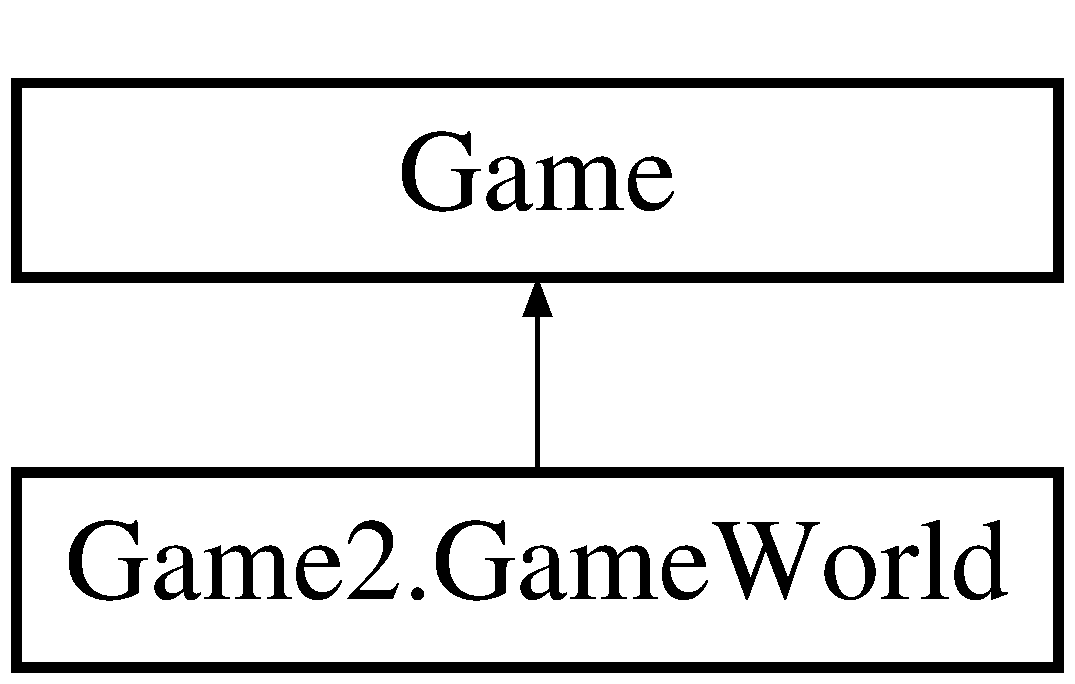
\includegraphics[height=2.000000cm]{class_game2_1_1_game_world}
\end{center}
\end{figure}
\subsection*{Public Member Functions}
\begin{DoxyCompactItemize}
\item 
\mbox{\hyperlink{class_game2_1_1_game_world_acecdd046d813514fe4a381fac3392417}{Game\+World}} ()
\item 
void \mbox{\hyperlink{class_game2_1_1_game_world_a268f162de7a1df8df00d740342465e41}{Spawn\+Enemies}} (double spawn\+Circle)
\begin{DoxyCompactList}\small\item\em Spawn Enemies and the boss also sets level based on wave time \end{DoxyCompactList}\item 
void \mbox{\hyperlink{class_game2_1_1_game_world_aa7f3f55732bc5adbd85898bb55523bad}{Spawn\+Boss}} (double spawn\+Circle, int ammount\+Boss)
\item 
void \mbox{\hyperlink{class_game2_1_1_game_world_a562424129dedeb22c5cc98d7a3f45a70}{Setlevel}} (int Wavetime\+Output)
\end{DoxyCompactItemize}
\subsection*{Static Public Member Functions}
\begin{DoxyCompactItemize}
\item 
static void \mbox{\hyperlink{class_game2_1_1_game_world_acde506006de6e0361c5175597cb07df2}{add\+Kill}} ()
\item 
static void \mbox{\hyperlink{class_game2_1_1_game_world_a5ab430402255839068ec6c074a827f10}{Deal\+Damnge\+To\+Player}} (int damnge)
\item 
static void \mbox{\hyperlink{class_game2_1_1_game_world_a39e2b721c387b979bf3b71cae226607d}{Add\+Game\+Object}} (\mbox{\hyperlink{class_game2_1_1_game_object}{Game\+Object}} go)
\item 
static void \mbox{\hyperlink{class_game2_1_1_game_world_a65a39808ffc51f5dbda1e3af966af50e}{Add\+E\+Ffect}} (\mbox{\hyperlink{class_game2_1_1_game_object}{Game\+Object}} go)
\item 
static void \mbox{\hyperlink{class_game2_1_1_game_world_a00bb1f85c2b674fe4a6b06b6887859cc}{Remove\+Game\+Object}} (\mbox{\hyperlink{class_game2_1_1_game_object}{Game\+Object}} go)
\end{DoxyCompactItemize}
\subsection*{Public Attributes}
\begin{DoxyCompactItemize}
\item 
List$<$ \mbox{\hyperlink{class_game2_1_1_game_object}{Game\+Object}} $>$ \mbox{\hyperlink{class_game2_1_1_game_world_a8843df0d3c8de0ca7c7f37f9cebce878}{game\+Objects}} = new List$<$\mbox{\hyperlink{class_game2_1_1_game_object}{Game\+Object}}$>$()
\item 
List$<$ \mbox{\hyperlink{class_game2_1_1_game_object}{Game\+Object}} $>$ \mbox{\hyperlink{class_game2_1_1_game_world_a7c01e067c7488bd5a80b810c5183e3af}{Effects}} = new List$<$\mbox{\hyperlink{class_game2_1_1_game_object}{Game\+Object}}$>$()
\end{DoxyCompactItemize}
\subsection*{Protected Member Functions}
\begin{DoxyCompactItemize}
\item 
override void \mbox{\hyperlink{class_game2_1_1_game_world_a8488fd97f682ca3cc0d3defe5094bb7f}{Initialize}} ()
\begin{DoxyCompactList}\small\item\em Allows the game to perform any initialization it needs to before starting to run. This is where it can query for any required services and load any non-\/graphic related content. Calling base.\+Initialize will enumerate through any components and initialize them as well. \end{DoxyCompactList}\item 
override void \mbox{\hyperlink{class_game2_1_1_game_world_a4bf53e37ff1497b08076b29ba9cc6494}{Load\+Content}} ()
\begin{DoxyCompactList}\small\item\em Load\+Content will be called once per game and is the place to load all of your content. \end{DoxyCompactList}\item 
override void \mbox{\hyperlink{class_game2_1_1_game_world_a653a301b00ac7b3fd16260d5c30d8f36}{Update}} (Game\+Time game\+Time)
\begin{DoxyCompactList}\small\item\em Allows the game to run logic such as updating the world, levels, checking for collisions, gathering input, and playing audio. \end{DoxyCompactList}\item 
override void \mbox{\hyperlink{class_game2_1_1_game_world_a2d3b767def6473b528eb4ea3bf54e37d}{Draw}} (Game\+Time game\+Time)
\begin{DoxyCompactList}\small\item\em This is called when the game should draw itself. \end{DoxyCompactList}\end{DoxyCompactItemize}
\subsection*{Properties}
\begin{DoxyCompactItemize}
\item 
int \mbox{\hyperlink{class_game2_1_1_game_world_a8289db0e2223e4d88fca02dd8a4281b3}{Healh\+Hold}}\hspace{0.3cm}{\ttfamily  \mbox{[}get\mbox{]}}
\item 
int \mbox{\hyperlink{class_game2_1_1_game_world_a9a7020d26597ee1ff08e5ade7686a482}{Kills}}\hspace{0.3cm}{\ttfamily  \mbox{[}get\mbox{]}}
\item 
static Rectangle \mbox{\hyperlink{class_game2_1_1_game_world_a33e4b367438dde0cb88d9fab8439c0e5}{Screen\+Size}}\hspace{0.3cm}{\ttfamily  \mbox{[}get\mbox{]}}
\end{DoxyCompactItemize}


\subsection{Detailed Description}
This is the main type for your game. 



\subsection{Constructor \& Destructor Documentation}
\mbox{\Hypertarget{class_game2_1_1_game_world_acecdd046d813514fe4a381fac3392417}\label{class_game2_1_1_game_world_acecdd046d813514fe4a381fac3392417}} 
\index{Game2\+::\+Game\+World@{Game2\+::\+Game\+World}!Game\+World@{Game\+World}}
\index{Game\+World@{Game\+World}!Game2\+::\+Game\+World@{Game2\+::\+Game\+World}}
\subsubsection{\texorpdfstring{Game\+World()}{GameWorld()}}
{\footnotesize\ttfamily Game2.\+Game\+World.\+Game\+World (\begin{DoxyParamCaption}{ }\end{DoxyParamCaption})}



\subsection{Member Function Documentation}
\mbox{\Hypertarget{class_game2_1_1_game_world_a65a39808ffc51f5dbda1e3af966af50e}\label{class_game2_1_1_game_world_a65a39808ffc51f5dbda1e3af966af50e}} 
\index{Game2\+::\+Game\+World@{Game2\+::\+Game\+World}!Add\+E\+Ffect@{Add\+E\+Ffect}}
\index{Add\+E\+Ffect@{Add\+E\+Ffect}!Game2\+::\+Game\+World@{Game2\+::\+Game\+World}}
\subsubsection{\texorpdfstring{Add\+E\+Ffect()}{AddEFfect()}}
{\footnotesize\ttfamily static void Game2.\+Game\+World.\+Add\+E\+Ffect (\begin{DoxyParamCaption}\item[{\mbox{\hyperlink{class_game2_1_1_game_object}{Game\+Object}}}]{go }\end{DoxyParamCaption})\hspace{0.3cm}{\ttfamily [static]}}

\mbox{\Hypertarget{class_game2_1_1_game_world_a39e2b721c387b979bf3b71cae226607d}\label{class_game2_1_1_game_world_a39e2b721c387b979bf3b71cae226607d}} 
\index{Game2\+::\+Game\+World@{Game2\+::\+Game\+World}!Add\+Game\+Object@{Add\+Game\+Object}}
\index{Add\+Game\+Object@{Add\+Game\+Object}!Game2\+::\+Game\+World@{Game2\+::\+Game\+World}}
\subsubsection{\texorpdfstring{Add\+Game\+Object()}{AddGameObject()}}
{\footnotesize\ttfamily static void Game2.\+Game\+World.\+Add\+Game\+Object (\begin{DoxyParamCaption}\item[{\mbox{\hyperlink{class_game2_1_1_game_object}{Game\+Object}}}]{go }\end{DoxyParamCaption})\hspace{0.3cm}{\ttfamily [static]}}

\mbox{\Hypertarget{class_game2_1_1_game_world_acde506006de6e0361c5175597cb07df2}\label{class_game2_1_1_game_world_acde506006de6e0361c5175597cb07df2}} 
\index{Game2\+::\+Game\+World@{Game2\+::\+Game\+World}!add\+Kill@{add\+Kill}}
\index{add\+Kill@{add\+Kill}!Game2\+::\+Game\+World@{Game2\+::\+Game\+World}}
\subsubsection{\texorpdfstring{add\+Kill()}{addKill()}}
{\footnotesize\ttfamily static void Game2.\+Game\+World.\+add\+Kill (\begin{DoxyParamCaption}{ }\end{DoxyParamCaption})\hspace{0.3cm}{\ttfamily [static]}}

\mbox{\Hypertarget{class_game2_1_1_game_world_a5ab430402255839068ec6c074a827f10}\label{class_game2_1_1_game_world_a5ab430402255839068ec6c074a827f10}} 
\index{Game2\+::\+Game\+World@{Game2\+::\+Game\+World}!Deal\+Damnge\+To\+Player@{Deal\+Damnge\+To\+Player}}
\index{Deal\+Damnge\+To\+Player@{Deal\+Damnge\+To\+Player}!Game2\+::\+Game\+World@{Game2\+::\+Game\+World}}
\subsubsection{\texorpdfstring{Deal\+Damnge\+To\+Player()}{DealDamngeToPlayer()}}
{\footnotesize\ttfamily static void Game2.\+Game\+World.\+Deal\+Damnge\+To\+Player (\begin{DoxyParamCaption}\item[{int}]{damnge }\end{DoxyParamCaption})\hspace{0.3cm}{\ttfamily [static]}}

\mbox{\Hypertarget{class_game2_1_1_game_world_a2d3b767def6473b528eb4ea3bf54e37d}\label{class_game2_1_1_game_world_a2d3b767def6473b528eb4ea3bf54e37d}} 
\index{Game2\+::\+Game\+World@{Game2\+::\+Game\+World}!Draw@{Draw}}
\index{Draw@{Draw}!Game2\+::\+Game\+World@{Game2\+::\+Game\+World}}
\subsubsection{\texorpdfstring{Draw()}{Draw()}}
{\footnotesize\ttfamily override void Game2.\+Game\+World.\+Draw (\begin{DoxyParamCaption}\item[{Game\+Time}]{game\+Time }\end{DoxyParamCaption})\hspace{0.3cm}{\ttfamily [protected]}}



This is called when the game should draw itself. 


\begin{DoxyParams}{Parameters}
{\em game\+Time} & Provides a snapshot of timing values.\\
\hline
\end{DoxyParams}
\mbox{\Hypertarget{class_game2_1_1_game_world_a8488fd97f682ca3cc0d3defe5094bb7f}\label{class_game2_1_1_game_world_a8488fd97f682ca3cc0d3defe5094bb7f}} 
\index{Game2\+::\+Game\+World@{Game2\+::\+Game\+World}!Initialize@{Initialize}}
\index{Initialize@{Initialize}!Game2\+::\+Game\+World@{Game2\+::\+Game\+World}}
\subsubsection{\texorpdfstring{Initialize()}{Initialize()}}
{\footnotesize\ttfamily override void Game2.\+Game\+World.\+Initialize (\begin{DoxyParamCaption}{ }\end{DoxyParamCaption})\hspace{0.3cm}{\ttfamily [protected]}}



Allows the game to perform any initialization it needs to before starting to run. This is where it can query for any required services and load any non-\/graphic related content. Calling base.\+Initialize will enumerate through any components and initialize them as well. 

\mbox{\Hypertarget{class_game2_1_1_game_world_a4bf53e37ff1497b08076b29ba9cc6494}\label{class_game2_1_1_game_world_a4bf53e37ff1497b08076b29ba9cc6494}} 
\index{Game2\+::\+Game\+World@{Game2\+::\+Game\+World}!Load\+Content@{Load\+Content}}
\index{Load\+Content@{Load\+Content}!Game2\+::\+Game\+World@{Game2\+::\+Game\+World}}
\subsubsection{\texorpdfstring{Load\+Content()}{LoadContent()}}
{\footnotesize\ttfamily override void Game2.\+Game\+World.\+Load\+Content (\begin{DoxyParamCaption}{ }\end{DoxyParamCaption})\hspace{0.3cm}{\ttfamily [protected]}}



Load\+Content will be called once per game and is the place to load all of your content. 

\mbox{\Hypertarget{class_game2_1_1_game_world_a00bb1f85c2b674fe4a6b06b6887859cc}\label{class_game2_1_1_game_world_a00bb1f85c2b674fe4a6b06b6887859cc}} 
\index{Game2\+::\+Game\+World@{Game2\+::\+Game\+World}!Remove\+Game\+Object@{Remove\+Game\+Object}}
\index{Remove\+Game\+Object@{Remove\+Game\+Object}!Game2\+::\+Game\+World@{Game2\+::\+Game\+World}}
\subsubsection{\texorpdfstring{Remove\+Game\+Object()}{RemoveGameObject()}}
{\footnotesize\ttfamily static void Game2.\+Game\+World.\+Remove\+Game\+Object (\begin{DoxyParamCaption}\item[{\mbox{\hyperlink{class_game2_1_1_game_object}{Game\+Object}}}]{go }\end{DoxyParamCaption})\hspace{0.3cm}{\ttfamily [static]}}

\mbox{\Hypertarget{class_game2_1_1_game_world_a562424129dedeb22c5cc98d7a3f45a70}\label{class_game2_1_1_game_world_a562424129dedeb22c5cc98d7a3f45a70}} 
\index{Game2\+::\+Game\+World@{Game2\+::\+Game\+World}!Setlevel@{Setlevel}}
\index{Setlevel@{Setlevel}!Game2\+::\+Game\+World@{Game2\+::\+Game\+World}}
\subsubsection{\texorpdfstring{Setlevel()}{Setlevel()}}
{\footnotesize\ttfamily void Game2.\+Game\+World.\+Setlevel (\begin{DoxyParamCaption}\item[{int}]{Wavetime\+Output }\end{DoxyParamCaption})}

\mbox{\Hypertarget{class_game2_1_1_game_world_aa7f3f55732bc5adbd85898bb55523bad}\label{class_game2_1_1_game_world_aa7f3f55732bc5adbd85898bb55523bad}} 
\index{Game2\+::\+Game\+World@{Game2\+::\+Game\+World}!Spawn\+Boss@{Spawn\+Boss}}
\index{Spawn\+Boss@{Spawn\+Boss}!Game2\+::\+Game\+World@{Game2\+::\+Game\+World}}
\subsubsection{\texorpdfstring{Spawn\+Boss()}{SpawnBoss()}}
{\footnotesize\ttfamily void Game2.\+Game\+World.\+Spawn\+Boss (\begin{DoxyParamCaption}\item[{double}]{spawn\+Circle,  }\item[{int}]{ammount\+Boss }\end{DoxyParamCaption})}

\mbox{\Hypertarget{class_game2_1_1_game_world_a268f162de7a1df8df00d740342465e41}\label{class_game2_1_1_game_world_a268f162de7a1df8df00d740342465e41}} 
\index{Game2\+::\+Game\+World@{Game2\+::\+Game\+World}!Spawn\+Enemies@{Spawn\+Enemies}}
\index{Spawn\+Enemies@{Spawn\+Enemies}!Game2\+::\+Game\+World@{Game2\+::\+Game\+World}}
\subsubsection{\texorpdfstring{Spawn\+Enemies()}{SpawnEnemies()}}
{\footnotesize\ttfamily void Game2.\+Game\+World.\+Spawn\+Enemies (\begin{DoxyParamCaption}\item[{double}]{spawn\+Circle }\end{DoxyParamCaption})}



Spawn Enemies and the boss also sets level based on wave time 

\mbox{\Hypertarget{class_game2_1_1_game_world_a653a301b00ac7b3fd16260d5c30d8f36}\label{class_game2_1_1_game_world_a653a301b00ac7b3fd16260d5c30d8f36}} 
\index{Game2\+::\+Game\+World@{Game2\+::\+Game\+World}!Update@{Update}}
\index{Update@{Update}!Game2\+::\+Game\+World@{Game2\+::\+Game\+World}}
\subsubsection{\texorpdfstring{Update()}{Update()}}
{\footnotesize\ttfamily override void Game2.\+Game\+World.\+Update (\begin{DoxyParamCaption}\item[{Game\+Time}]{game\+Time }\end{DoxyParamCaption})\hspace{0.3cm}{\ttfamily [protected]}}



Allows the game to run logic such as updating the world, levels, checking for collisions, gathering input, and playing audio. 


\begin{DoxyParams}{Parameters}
{\em game\+Time} & Provides a snapshot of timing values.\\
\hline
\end{DoxyParams}


\subsection{Member Data Documentation}
\mbox{\Hypertarget{class_game2_1_1_game_world_a7c01e067c7488bd5a80b810c5183e3af}\label{class_game2_1_1_game_world_a7c01e067c7488bd5a80b810c5183e3af}} 
\index{Game2\+::\+Game\+World@{Game2\+::\+Game\+World}!Effects@{Effects}}
\index{Effects@{Effects}!Game2\+::\+Game\+World@{Game2\+::\+Game\+World}}
\subsubsection{\texorpdfstring{Effects}{Effects}}
{\footnotesize\ttfamily List$<$\mbox{\hyperlink{class_game2_1_1_game_object}{Game\+Object}}$>$ Game2.\+Game\+World.\+Effects = new List$<$\mbox{\hyperlink{class_game2_1_1_game_object}{Game\+Object}}$>$()}

\mbox{\Hypertarget{class_game2_1_1_game_world_a8843df0d3c8de0ca7c7f37f9cebce878}\label{class_game2_1_1_game_world_a8843df0d3c8de0ca7c7f37f9cebce878}} 
\index{Game2\+::\+Game\+World@{Game2\+::\+Game\+World}!game\+Objects@{game\+Objects}}
\index{game\+Objects@{game\+Objects}!Game2\+::\+Game\+World@{Game2\+::\+Game\+World}}
\subsubsection{\texorpdfstring{game\+Objects}{gameObjects}}
{\footnotesize\ttfamily List$<$\mbox{\hyperlink{class_game2_1_1_game_object}{Game\+Object}}$>$ Game2.\+Game\+World.\+game\+Objects = new List$<$\mbox{\hyperlink{class_game2_1_1_game_object}{Game\+Object}}$>$()}



\subsection{Property Documentation}
\mbox{\Hypertarget{class_game2_1_1_game_world_a8289db0e2223e4d88fca02dd8a4281b3}\label{class_game2_1_1_game_world_a8289db0e2223e4d88fca02dd8a4281b3}} 
\index{Game2\+::\+Game\+World@{Game2\+::\+Game\+World}!Healh\+Hold@{Healh\+Hold}}
\index{Healh\+Hold@{Healh\+Hold}!Game2\+::\+Game\+World@{Game2\+::\+Game\+World}}
\subsubsection{\texorpdfstring{Healh\+Hold}{HealhHold}}
{\footnotesize\ttfamily int Game2.\+Game\+World.\+Healh\+Hold\hspace{0.3cm}{\ttfamily [get]}}

\mbox{\Hypertarget{class_game2_1_1_game_world_a9a7020d26597ee1ff08e5ade7686a482}\label{class_game2_1_1_game_world_a9a7020d26597ee1ff08e5ade7686a482}} 
\index{Game2\+::\+Game\+World@{Game2\+::\+Game\+World}!Kills@{Kills}}
\index{Kills@{Kills}!Game2\+::\+Game\+World@{Game2\+::\+Game\+World}}
\subsubsection{\texorpdfstring{Kills}{Kills}}
{\footnotesize\ttfamily int Game2.\+Game\+World.\+Kills\hspace{0.3cm}{\ttfamily [get]}}

\mbox{\Hypertarget{class_game2_1_1_game_world_a33e4b367438dde0cb88d9fab8439c0e5}\label{class_game2_1_1_game_world_a33e4b367438dde0cb88d9fab8439c0e5}} 
\index{Game2\+::\+Game\+World@{Game2\+::\+Game\+World}!Screen\+Size@{Screen\+Size}}
\index{Screen\+Size@{Screen\+Size}!Game2\+::\+Game\+World@{Game2\+::\+Game\+World}}
\subsubsection{\texorpdfstring{Screen\+Size}{ScreenSize}}
{\footnotesize\ttfamily Rectangle Game2.\+Game\+World.\+Screen\+Size\hspace{0.3cm}{\ttfamily [static]}, {\ttfamily [get]}}



The documentation for this class was generated from the following file\+:\begin{DoxyCompactItemize}
\item 
Game2/\mbox{\hyperlink{_game_world_8cs}{Game\+World.\+cs}}\end{DoxyCompactItemize}

\hypertarget{class_game2_1_1_player}{}\section{Game2.\+Player Class Reference}
\label{class_game2_1_1_player}\index{Game2.\+Player@{Game2.\+Player}}


Class that represents the player  


Inheritance diagram for Game2.\+Player\+:\begin{figure}[H]
\begin{center}
\leavevmode
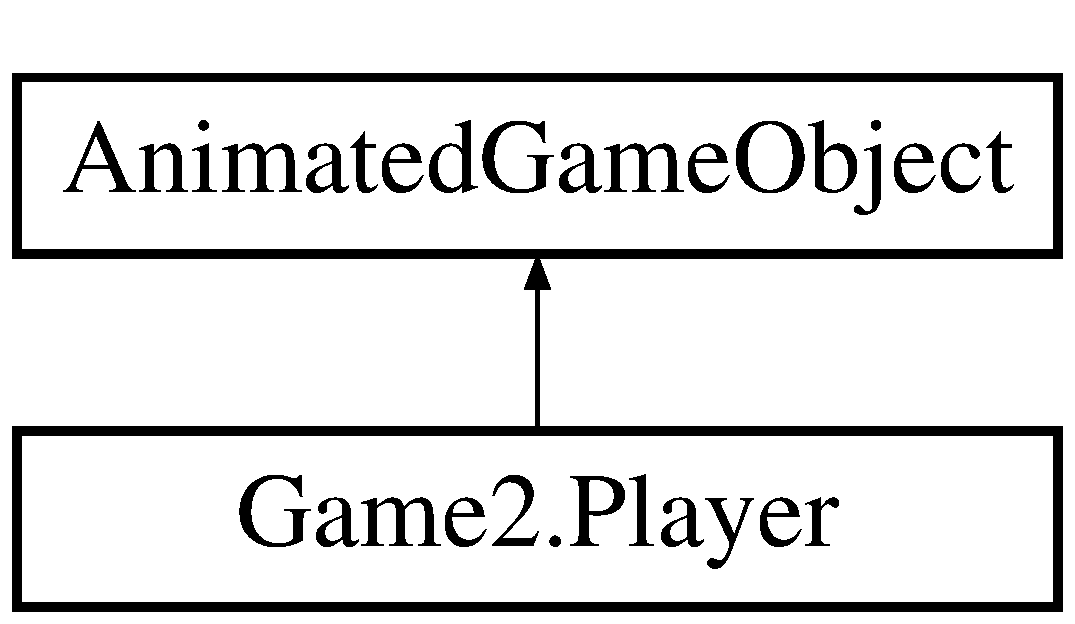
\includegraphics[height=2.000000cm]{class_game2_1_1_player}
\end{center}
\end{figure}
\subsection*{Public Member Functions}
\begin{DoxyCompactItemize}
\item 
\mbox{\hyperlink{class_game2_1_1_player_aba2289750066d1fbf0cf9ba5aabf7027}{Player}} (Content\+Manager content)
\begin{DoxyCompactList}\small\item\em Sets the player stats and health \end{DoxyCompactList}\item 
override void \mbox{\hyperlink{class_game2_1_1_player_a14ef301313a531bd8379300ef0588378}{Update}} (Game\+Time game\+Time)
\begin{DoxyCompactList}\small\item\em Sets controls mouse and keyboard, aswell as rotation and gun sound effect \end{DoxyCompactList}\end{DoxyCompactItemize}
\subsection*{Public Attributes}
\begin{DoxyCompactItemize}
\item 
Vector2 \mbox{\hyperlink{class_game2_1_1_player_ae8c457659c53b82a059739f18c52de9c}{direction}} = new Vector2()
\end{DoxyCompactItemize}
\subsection*{Properties}
\begin{DoxyCompactItemize}
\item 
int \mbox{\hyperlink{class_game2_1_1_player_a0de12ae1963fa77b943c0da0c41d9a38}{Kill\+Count}}\hspace{0.3cm}{\ttfamily  \mbox{[}get\mbox{]}}
\item 
Vector2 \mbox{\hyperlink{class_game2_1_1_player_a03cfdc80acd38082853948af2f299824}{player\+Position}}\hspace{0.3cm}{\ttfamily  \mbox{[}get\mbox{]}}
\item 
int \mbox{\hyperlink{class_game2_1_1_player_a0f289bb7a69b375f4c0bb7bf5ab87430}{Health}}\hspace{0.3cm}{\ttfamily  \mbox{[}get, set\mbox{]}}
\end{DoxyCompactItemize}


\subsection{Detailed Description}
Class that represents the player 



\subsection{Constructor \& Destructor Documentation}
\mbox{\Hypertarget{class_game2_1_1_player_aba2289750066d1fbf0cf9ba5aabf7027}\label{class_game2_1_1_player_aba2289750066d1fbf0cf9ba5aabf7027}} 
\index{Game2\+::\+Player@{Game2\+::\+Player}!Player@{Player}}
\index{Player@{Player}!Game2\+::\+Player@{Game2\+::\+Player}}
\subsubsection{\texorpdfstring{Player()}{Player()}}
{\footnotesize\ttfamily Game2.\+Player.\+Player (\begin{DoxyParamCaption}\item[{Content\+Manager}]{content }\end{DoxyParamCaption})}



Sets the player stats and health 


\begin{DoxyParams}{Parameters}
{\em content} & \\
\hline
\end{DoxyParams}


\subsection{Member Function Documentation}
\mbox{\Hypertarget{class_game2_1_1_player_a14ef301313a531bd8379300ef0588378}\label{class_game2_1_1_player_a14ef301313a531bd8379300ef0588378}} 
\index{Game2\+::\+Player@{Game2\+::\+Player}!Update@{Update}}
\index{Update@{Update}!Game2\+::\+Player@{Game2\+::\+Player}}
\subsubsection{\texorpdfstring{Update()}{Update()}}
{\footnotesize\ttfamily override void Game2.\+Player.\+Update (\begin{DoxyParamCaption}\item[{Game\+Time}]{game\+Time }\end{DoxyParamCaption})}



Sets controls mouse and keyboard, aswell as rotation and gun sound effect 


\begin{DoxyParams}{Parameters}
{\em game\+Time} & \\
\hline
\end{DoxyParams}


\subsection{Member Data Documentation}
\mbox{\Hypertarget{class_game2_1_1_player_ae8c457659c53b82a059739f18c52de9c}\label{class_game2_1_1_player_ae8c457659c53b82a059739f18c52de9c}} 
\index{Game2\+::\+Player@{Game2\+::\+Player}!direction@{direction}}
\index{direction@{direction}!Game2\+::\+Player@{Game2\+::\+Player}}
\subsubsection{\texorpdfstring{direction}{direction}}
{\footnotesize\ttfamily Vector2 Game2.\+Player.\+direction = new Vector2()}



\subsection{Property Documentation}
\mbox{\Hypertarget{class_game2_1_1_player_a0f289bb7a69b375f4c0bb7bf5ab87430}\label{class_game2_1_1_player_a0f289bb7a69b375f4c0bb7bf5ab87430}} 
\index{Game2\+::\+Player@{Game2\+::\+Player}!Health@{Health}}
\index{Health@{Health}!Game2\+::\+Player@{Game2\+::\+Player}}
\subsubsection{\texorpdfstring{Health}{Health}}
{\footnotesize\ttfamily int Game2.\+Player.\+Health\hspace{0.3cm}{\ttfamily [get]}, {\ttfamily [set]}}

\mbox{\Hypertarget{class_game2_1_1_player_a0de12ae1963fa77b943c0da0c41d9a38}\label{class_game2_1_1_player_a0de12ae1963fa77b943c0da0c41d9a38}} 
\index{Game2\+::\+Player@{Game2\+::\+Player}!Kill\+Count@{Kill\+Count}}
\index{Kill\+Count@{Kill\+Count}!Game2\+::\+Player@{Game2\+::\+Player}}
\subsubsection{\texorpdfstring{Kill\+Count}{KillCount}}
{\footnotesize\ttfamily int Game2.\+Player.\+Kill\+Count\hspace{0.3cm}{\ttfamily [get]}}

\mbox{\Hypertarget{class_game2_1_1_player_a03cfdc80acd38082853948af2f299824}\label{class_game2_1_1_player_a03cfdc80acd38082853948af2f299824}} 
\index{Game2\+::\+Player@{Game2\+::\+Player}!player\+Position@{player\+Position}}
\index{player\+Position@{player\+Position}!Game2\+::\+Player@{Game2\+::\+Player}}
\subsubsection{\texorpdfstring{player\+Position}{playerPosition}}
{\footnotesize\ttfamily Vector2 Game2.\+Player.\+player\+Position\hspace{0.3cm}{\ttfamily [get]}}



The documentation for this class was generated from the following file\+:\begin{DoxyCompactItemize}
\item 
\mbox{\hyperlink{_player_8cs}{Player.\+cs}}\end{DoxyCompactItemize}

\hypertarget{class_game2_1_1_player_blood}{}\section{Game2.\+Player\+Blood Class Reference}
\label{class_game2_1_1_player_blood}\index{Game2.\+Player\+Blood@{Game2.\+Player\+Blood}}
Inheritance diagram for Game2.\+Player\+Blood\+:\begin{figure}[H]
\begin{center}
\leavevmode
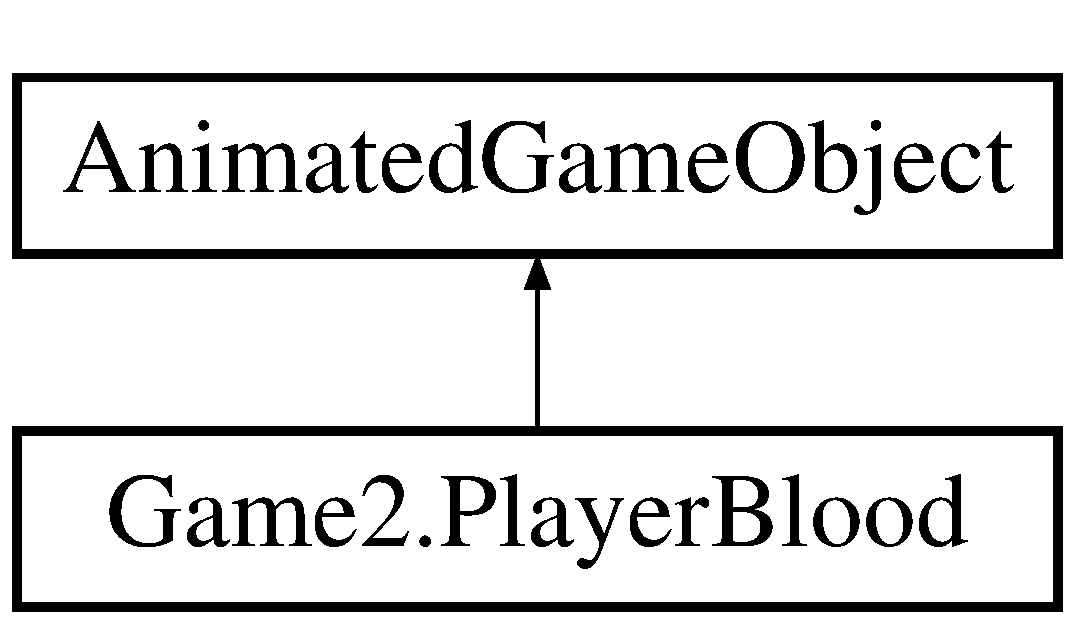
\includegraphics[height=2.000000cm]{class_game2_1_1_player_blood}
\end{center}
\end{figure}
\subsection*{Public Member Functions}
\begin{DoxyCompactItemize}
\item 
\mbox{\hyperlink{class_game2_1_1_player_blood_a353c696afecffe2fd3dc22d2d15f14bb}{Player\+Blood}} (int size, Vector2 start\+Position, Content\+Manager content)
\begin{DoxyCompactList}\small\item\em Adds blood effect when zombies walk into player \end{DoxyCompactList}\item 
override void \mbox{\hyperlink{class_game2_1_1_player_blood_a165cc6d8cf92da781ba21ce9cabca5be}{Update}} (Game\+Time game\+Time)
\end{DoxyCompactItemize}


\subsection{Constructor \& Destructor Documentation}
\mbox{\Hypertarget{class_game2_1_1_player_blood_a353c696afecffe2fd3dc22d2d15f14bb}\label{class_game2_1_1_player_blood_a353c696afecffe2fd3dc22d2d15f14bb}} 
\index{Game2\+::\+Player\+Blood@{Game2\+::\+Player\+Blood}!Player\+Blood@{Player\+Blood}}
\index{Player\+Blood@{Player\+Blood}!Game2\+::\+Player\+Blood@{Game2\+::\+Player\+Blood}}
\subsubsection{\texorpdfstring{Player\+Blood()}{PlayerBlood()}}
{\footnotesize\ttfamily Game2.\+Player\+Blood.\+Player\+Blood (\begin{DoxyParamCaption}\item[{int}]{size,  }\item[{Vector2}]{start\+Position,  }\item[{Content\+Manager}]{content }\end{DoxyParamCaption})}



Adds blood effect when zombies walk into player 


\begin{DoxyParams}{Parameters}
{\em size} & \\
\hline
{\em start\+Position} & \\
\hline
{\em content} & \\
\hline
\end{DoxyParams}


\subsection{Member Function Documentation}
\mbox{\Hypertarget{class_game2_1_1_player_blood_a165cc6d8cf92da781ba21ce9cabca5be}\label{class_game2_1_1_player_blood_a165cc6d8cf92da781ba21ce9cabca5be}} 
\index{Game2\+::\+Player\+Blood@{Game2\+::\+Player\+Blood}!Update@{Update}}
\index{Update@{Update}!Game2\+::\+Player\+Blood@{Game2\+::\+Player\+Blood}}
\subsubsection{\texorpdfstring{Update()}{Update()}}
{\footnotesize\ttfamily override void Game2.\+Player\+Blood.\+Update (\begin{DoxyParamCaption}\item[{Game\+Time}]{game\+Time }\end{DoxyParamCaption})}



The documentation for this class was generated from the following file\+:\begin{DoxyCompactItemize}
\item 
Game2/\mbox{\hyperlink{_player_blood_8cs}{Player\+Blood.\+cs}}\end{DoxyCompactItemize}

\hypertarget{class_solar_battle_1_1_camera_1_1_player_camera}{}\section{Solar\+Battle.\+Camera.\+Player\+Camera Class Reference}
\label{class_solar_battle_1_1_camera_1_1_player_camera}\index{Solar\+Battle.\+Camera.\+Player\+Camera@{Solar\+Battle.\+Camera.\+Player\+Camera}}
\subsection*{Public Member Functions}
\begin{DoxyCompactItemize}
\item 
\mbox{\hyperlink{class_solar_battle_1_1_camera_1_1_player_camera_ab617c8888645482072dc9b983d8a5d6e}{Player\+Camera}} (Viewport view, float scale)
\item 
void \mbox{\hyperlink{class_solar_battle_1_1_camera_1_1_player_camera_ab2ba554b5610da18c104238f3529d074}{Update}} (Player\+Ship player)
\item 
Matrix \mbox{\hyperlink{class_solar_battle_1_1_camera_1_1_player_camera_a13bd90207a9d212b549871dc790849dc}{get\+Transform}} ()
\item 
Vector2 \mbox{\hyperlink{class_solar_battle_1_1_camera_1_1_player_camera_af3a0cf6ebdedd4932b8961f457fd279e}{get\+Camera\+Focus}} ()
\item 
float \mbox{\hyperlink{class_solar_battle_1_1_camera_1_1_player_camera_a1667a5cd6cbf37f2f0b9121b57476d52}{get\+Scale}} ()
\end{DoxyCompactItemize}
\subsection*{Public Attributes}
\begin{DoxyCompactItemize}
\item 
Matrix \mbox{\hyperlink{class_solar_battle_1_1_camera_1_1_player_camera_a6a863da393627c0df6176e4b69b9b106}{m\+\_\+transform}}
\end{DoxyCompactItemize}


\subsection{Constructor \& Destructor Documentation}
\mbox{\Hypertarget{class_solar_battle_1_1_camera_1_1_player_camera_ab617c8888645482072dc9b983d8a5d6e}\label{class_solar_battle_1_1_camera_1_1_player_camera_ab617c8888645482072dc9b983d8a5d6e}} 
\index{Solar\+Battle\+::\+Camera\+::\+Player\+Camera@{Solar\+Battle\+::\+Camera\+::\+Player\+Camera}!Player\+Camera@{Player\+Camera}}
\index{Player\+Camera@{Player\+Camera}!Solar\+Battle\+::\+Camera\+::\+Player\+Camera@{Solar\+Battle\+::\+Camera\+::\+Player\+Camera}}
\subsubsection{\texorpdfstring{Player\+Camera()}{PlayerCamera()}}
{\footnotesize\ttfamily Solar\+Battle.\+Camera.\+Player\+Camera.\+Player\+Camera (\begin{DoxyParamCaption}\item[{Viewport}]{view,  }\item[{float}]{scale }\end{DoxyParamCaption})}



\subsection{Member Function Documentation}
\mbox{\Hypertarget{class_solar_battle_1_1_camera_1_1_player_camera_af3a0cf6ebdedd4932b8961f457fd279e}\label{class_solar_battle_1_1_camera_1_1_player_camera_af3a0cf6ebdedd4932b8961f457fd279e}} 
\index{Solar\+Battle\+::\+Camera\+::\+Player\+Camera@{Solar\+Battle\+::\+Camera\+::\+Player\+Camera}!get\+Camera\+Focus@{get\+Camera\+Focus}}
\index{get\+Camera\+Focus@{get\+Camera\+Focus}!Solar\+Battle\+::\+Camera\+::\+Player\+Camera@{Solar\+Battle\+::\+Camera\+::\+Player\+Camera}}
\subsubsection{\texorpdfstring{get\+Camera\+Focus()}{getCameraFocus()}}
{\footnotesize\ttfamily Vector2 Solar\+Battle.\+Camera.\+Player\+Camera.\+get\+Camera\+Focus (\begin{DoxyParamCaption}{ }\end{DoxyParamCaption})}

\mbox{\Hypertarget{class_solar_battle_1_1_camera_1_1_player_camera_a1667a5cd6cbf37f2f0b9121b57476d52}\label{class_solar_battle_1_1_camera_1_1_player_camera_a1667a5cd6cbf37f2f0b9121b57476d52}} 
\index{Solar\+Battle\+::\+Camera\+::\+Player\+Camera@{Solar\+Battle\+::\+Camera\+::\+Player\+Camera}!get\+Scale@{get\+Scale}}
\index{get\+Scale@{get\+Scale}!Solar\+Battle\+::\+Camera\+::\+Player\+Camera@{Solar\+Battle\+::\+Camera\+::\+Player\+Camera}}
\subsubsection{\texorpdfstring{get\+Scale()}{getScale()}}
{\footnotesize\ttfamily float Solar\+Battle.\+Camera.\+Player\+Camera.\+get\+Scale (\begin{DoxyParamCaption}{ }\end{DoxyParamCaption})}

\mbox{\Hypertarget{class_solar_battle_1_1_camera_1_1_player_camera_a13bd90207a9d212b549871dc790849dc}\label{class_solar_battle_1_1_camera_1_1_player_camera_a13bd90207a9d212b549871dc790849dc}} 
\index{Solar\+Battle\+::\+Camera\+::\+Player\+Camera@{Solar\+Battle\+::\+Camera\+::\+Player\+Camera}!get\+Transform@{get\+Transform}}
\index{get\+Transform@{get\+Transform}!Solar\+Battle\+::\+Camera\+::\+Player\+Camera@{Solar\+Battle\+::\+Camera\+::\+Player\+Camera}}
\subsubsection{\texorpdfstring{get\+Transform()}{getTransform()}}
{\footnotesize\ttfamily Matrix Solar\+Battle.\+Camera.\+Player\+Camera.\+get\+Transform (\begin{DoxyParamCaption}{ }\end{DoxyParamCaption})}

\mbox{\Hypertarget{class_solar_battle_1_1_camera_1_1_player_camera_ab2ba554b5610da18c104238f3529d074}\label{class_solar_battle_1_1_camera_1_1_player_camera_ab2ba554b5610da18c104238f3529d074}} 
\index{Solar\+Battle\+::\+Camera\+::\+Player\+Camera@{Solar\+Battle\+::\+Camera\+::\+Player\+Camera}!Update@{Update}}
\index{Update@{Update}!Solar\+Battle\+::\+Camera\+::\+Player\+Camera@{Solar\+Battle\+::\+Camera\+::\+Player\+Camera}}
\subsubsection{\texorpdfstring{Update()}{Update()}}
{\footnotesize\ttfamily void Solar\+Battle.\+Camera.\+Player\+Camera.\+Update (\begin{DoxyParamCaption}\item[{Player\+Ship}]{player }\end{DoxyParamCaption})}



\subsection{Member Data Documentation}
\mbox{\Hypertarget{class_solar_battle_1_1_camera_1_1_player_camera_a6a863da393627c0df6176e4b69b9b106}\label{class_solar_battle_1_1_camera_1_1_player_camera_a6a863da393627c0df6176e4b69b9b106}} 
\index{Solar\+Battle\+::\+Camera\+::\+Player\+Camera@{Solar\+Battle\+::\+Camera\+::\+Player\+Camera}!m\+\_\+transform@{m\+\_\+transform}}
\index{m\+\_\+transform@{m\+\_\+transform}!Solar\+Battle\+::\+Camera\+::\+Player\+Camera@{Solar\+Battle\+::\+Camera\+::\+Player\+Camera}}
\subsubsection{\texorpdfstring{m\+\_\+transform}{m\_transform}}
{\footnotesize\ttfamily Matrix Solar\+Battle.\+Camera.\+Player\+Camera.\+m\+\_\+transform}



The documentation for this class was generated from the following file\+:\begin{DoxyCompactItemize}
\item 
\mbox{\hyperlink{_player_camera_8cs}{Player\+Camera.\+cs}}\end{DoxyCompactItemize}

\hypertarget{class_game2_1_1test}{}\section{Game2.\+test Class Reference}
\label{class_game2_1_1test}\index{Game2.\+test@{Game2.\+test}}


The documentation for this class was generated from the following file\+:\begin{DoxyCompactItemize}
\item 
Game2/\mbox{\hyperlink{test_8cs}{test.\+cs}}\end{DoxyCompactItemize}

\chapter{File Documentation}
\hypertarget{_animated_game_object_8cs}{}\section{Game2/\+Animated\+Game\+Object.cs File Reference}
\label{_animated_game_object_8cs}\index{Game2/\+Animated\+Game\+Object.\+cs@{Game2/\+Animated\+Game\+Object.\+cs}}
\subsection*{Namespaces}
\begin{DoxyCompactItemize}
\item 
namespace \mbox{\hyperlink{namespace_game2}{Game2}}
\end{DoxyCompactItemize}

\hypertarget{_blood_8cs}{}\section{Game2/\+Blood.cs File Reference}
\label{_blood_8cs}\index{Game2/\+Blood.\+cs@{Game2/\+Blood.\+cs}}
\subsection*{Classes}
\begin{DoxyCompactItemize}
\item 
class \mbox{\hyperlink{class_game2_1_1_blood}{Game2.\+Blood}}
\end{DoxyCompactItemize}
\subsection*{Namespaces}
\begin{DoxyCompactItemize}
\item 
namespace \mbox{\hyperlink{namespace_game2}{Game2}}
\end{DoxyCompactItemize}

\hypertarget{_blood_effect_8cs}{}\section{Blood\+Effect.\+cs File Reference}
\label{_blood_effect_8cs}\index{Blood\+Effect.\+cs@{Blood\+Effect.\+cs}}
\subsection*{Classes}
\begin{DoxyCompactItemize}
\item 
class \mbox{\hyperlink{class_game2_1_1_blood_effect}{Game2.\+Blood\+Effect}}
\end{DoxyCompactItemize}
\subsection*{Namespaces}
\begin{DoxyCompactItemize}
\item 
namespace \mbox{\hyperlink{namespace_game2}{Game2}}
\end{DoxyCompactItemize}

\hypertarget{_boss_8cs}{}\section{Boss.\+cs File Reference}
\label{_boss_8cs}\index{Boss.\+cs@{Boss.\+cs}}
\subsection*{Classes}
\begin{DoxyCompactItemize}
\item 
class \mbox{\hyperlink{class_game2_1_1_boss}{Game2.\+Boss}}
\begin{DoxyCompactList}\small\item\em Class that represents a boss \end{DoxyCompactList}\end{DoxyCompactItemize}
\subsection*{Namespaces}
\begin{DoxyCompactItemize}
\item 
namespace \mbox{\hyperlink{namespace_game2}{Game2}}
\end{DoxyCompactItemize}

\hypertarget{_bullet_8cs}{}\section{Bullet.\+cs File Reference}
\label{_bullet_8cs}\index{Bullet.\+cs@{Bullet.\+cs}}
\subsection*{Classes}
\begin{DoxyCompactItemize}
\item 
class \mbox{\hyperlink{class_game2_1_1_bullet}{Game2.\+Bullet}}
\begin{DoxyCompactList}\small\item\em Class that represents a \mbox{\hyperlink{class_game2_1_1_bullet}{Bullet}} fired from the player \end{DoxyCompactList}\end{DoxyCompactItemize}
\subsection*{Namespaces}
\begin{DoxyCompactItemize}
\item 
namespace \mbox{\hyperlink{namespace_game2}{Game2}}
\end{DoxyCompactItemize}

\hypertarget{_enemy_8cs}{}\section{Game2/\+Enemy.cs File Reference}
\label{_enemy_8cs}\index{Game2/\+Enemy.\+cs@{Game2/\+Enemy.\+cs}}
\subsection*{Classes}
\begin{DoxyCompactItemize}
\item 
class \mbox{\hyperlink{class_game2_1_1_enemy}{Game2.\+Enemy}}
\begin{DoxyCompactList}\small\item\em Class that represents a zombie \end{DoxyCompactList}\end{DoxyCompactItemize}
\subsection*{Namespaces}
\begin{DoxyCompactItemize}
\item 
namespace \mbox{\hyperlink{namespace_game2}{Game2}}
\end{DoxyCompactItemize}

\hypertarget{_game_object_8cs}{}\section{Game\+Object.\+cs File Reference}
\label{_game_object_8cs}\index{Game\+Object.\+cs@{Game\+Object.\+cs}}
\subsection*{Classes}
\begin{DoxyCompactItemize}
\item 
class \mbox{\hyperlink{class_game2_1_1_game_object}{Game2.\+Game\+Object}}
\end{DoxyCompactItemize}
\subsection*{Namespaces}
\begin{DoxyCompactItemize}
\item 
namespace \mbox{\hyperlink{namespace_game2}{Game2}}
\end{DoxyCompactItemize}

\hypertarget{_game_over_menu_screen_8cs}{}\section{Game2/\+Game\+Over\+Menu\+Screen.cs File Reference}
\label{_game_over_menu_screen_8cs}\index{Game2/\+Game\+Over\+Menu\+Screen.\+cs@{Game2/\+Game\+Over\+Menu\+Screen.\+cs}}
\subsection*{Classes}
\begin{DoxyCompactItemize}
\item 
class \mbox{\hyperlink{class_game2_1_1_game_over_menu_screen}{Game2.\+Game\+Over\+Menu\+Screen}}
\end{DoxyCompactItemize}
\subsection*{Namespaces}
\begin{DoxyCompactItemize}
\item 
namespace \mbox{\hyperlink{namespace_game2}{Game2}}
\end{DoxyCompactItemize}

\hypertarget{_game_timer_8cs}{}\section{Game\+Timer.\+cs File Reference}
\label{_game_timer_8cs}\index{Game\+Timer.\+cs@{Game\+Timer.\+cs}}
\subsection*{Classes}
\begin{DoxyCompactItemize}
\item 
class \mbox{\hyperlink{class_game2_1_1_game_timer}{Game2.\+Game\+Timer}}
\begin{DoxyCompactList}\small\item\em Class that represents a game time to set waves \end{DoxyCompactList}\end{DoxyCompactItemize}
\subsection*{Namespaces}
\begin{DoxyCompactItemize}
\item 
namespace \mbox{\hyperlink{namespace_game2}{Game2}}
\end{DoxyCompactItemize}

\hypertarget{_game_world_8cs}{}\section{Game2/\+Game\+World.cs File Reference}
\label{_game_world_8cs}\index{Game2/\+Game\+World.\+cs@{Game2/\+Game\+World.\+cs}}
\subsection*{Classes}
\begin{DoxyCompactItemize}
\item 
class \mbox{\hyperlink{class_game2_1_1_game_world}{Game2.\+Game\+World}}
\begin{DoxyCompactList}\small\item\em This is the main type for your game. \end{DoxyCompactList}\end{DoxyCompactItemize}
\subsection*{Namespaces}
\begin{DoxyCompactItemize}
\item 
namespace \mbox{\hyperlink{namespace_game2}{Game2}}
\end{DoxyCompactItemize}

\hypertarget{_player_8cs}{}\section{Player.\+cs File Reference}
\label{_player_8cs}\index{Player.\+cs@{Player.\+cs}}
\subsection*{Classes}
\begin{DoxyCompactItemize}
\item 
class \mbox{\hyperlink{class_game2_1_1_player}{Game2.\+Player}}
\begin{DoxyCompactList}\small\item\em Class that represents the player \end{DoxyCompactList}\end{DoxyCompactItemize}
\subsection*{Namespaces}
\begin{DoxyCompactItemize}
\item 
namespace \mbox{\hyperlink{namespace_game2}{Game2}}
\end{DoxyCompactItemize}

\hypertarget{_player_blood_8cs}{}\section{Game2/\+Player\+Blood.cs File Reference}
\label{_player_blood_8cs}\index{Game2/\+Player\+Blood.\+cs@{Game2/\+Player\+Blood.\+cs}}
\subsection*{Classes}
\begin{DoxyCompactItemize}
\item 
class \mbox{\hyperlink{class_game2_1_1_player_blood}{Game2.\+Player\+Blood}}
\end{DoxyCompactItemize}
\subsection*{Namespaces}
\begin{DoxyCompactItemize}
\item 
namespace \mbox{\hyperlink{namespace_game2}{Game2}}
\end{DoxyCompactItemize}

\hypertarget{_player_camera_8cs}{}\section{Player\+Camera.\+cs File Reference}
\label{_player_camera_8cs}\index{Player\+Camera.\+cs@{Player\+Camera.\+cs}}
\subsection*{Classes}
\begin{DoxyCompactItemize}
\item 
class \mbox{\hyperlink{class_solar_battle_1_1_camera_1_1_player_camera}{Solar\+Battle.\+Camera.\+Player\+Camera}}
\end{DoxyCompactItemize}
\subsection*{Namespaces}
\begin{DoxyCompactItemize}
\item 
namespace \mbox{\hyperlink{namespace_solar_battle_1_1_camera}{Solar\+Battle.\+Camera}}
\end{DoxyCompactItemize}

\hypertarget{_program_8cs}{}\section{Game2/\+Program.cs File Reference}
\label{_program_8cs}\index{Game2/\+Program.\+cs@{Game2/\+Program.\+cs}}
\subsection*{Namespaces}
\begin{DoxyCompactItemize}
\item 
namespace \mbox{\hyperlink{namespace_game2}{Game2}}
\end{DoxyCompactItemize}

\hypertarget{test_8cs}{}\section{Game2/test.cs File Reference}
\label{test_8cs}\index{Game2/test.\+cs@{Game2/test.\+cs}}
\subsection*{Classes}
\begin{DoxyCompactItemize}
\item 
class \mbox{\hyperlink{class_game2_1_1test}{Game2.\+test}}
\end{DoxyCompactItemize}
\subsection*{Namespaces}
\begin{DoxyCompactItemize}
\item 
namespace \mbox{\hyperlink{namespace_game2}{Game2}}
\end{DoxyCompactItemize}

%--- End generated contents ---

% Index
\backmatter
\newpage
\phantomsection
\clearemptydoublepage
\addcontentsline{toc}{chapter}{Index}
\printindex

\end{document}
